\documentclass[11pt,a4paper]{article}

\usepackage[utf8]{inputenc}
\usepackage[T1]{fontenc}
\usepackage{mathpazo}
\usepackage{amsmath,amssymb,amsthm,mathtools,bm}
\usepackage[margin=2.4cm]{geometry}
\usepackage{xcolor}
\usepackage{booktabs,array,enumitem}
\usepackage{microtype}
\usepackage{tikz}
\usetikzlibrary{arrows.meta,positioning,calc,shapes.geometric,shapes.misc,fit,backgrounds,decorations.pathreplacing}
\usepackage{pgfplots}
\usepackage{float}
\usepgfplotslibrary{groupplots,fillbetween}
\pgfplotsset{compat=1.16}
\usepackage[most]{tcolorbox}
\usepackage[labelfont=bf,font=small]{caption}
\usepackage[colorlinks=true,linkcolor=blue!50!black,urlcolor=blue!50!black,citecolor=blue!50!black]{hyperref}

\setlist[itemize]{itemsep=2pt,topsep=3pt}
\setlist[enumerate]{itemsep=2pt,topsep=3pt}
\setlength{\parskip}{4pt}
\setlength{\parindent}{0pt}

% ------------------------------------------------------------------ macros
\newcommand{\E}{\mathbb{E}}
\newcommand{\Prob}{\mathbb{P}}
\newcommand{\Reg}{\mathrm{Regret}}
\newcommand{\Unif}{\mathrm{Unif}}
\newcommand{\ind}{\mathbf{1}}
\newcommand{\rh}{\hat{\mathbf{r}}}
\newcommand{\calA}{\mathcal{A}}
\newcommand{\calX}{\mathcal{X}}
\newcommand{\Norm}{\mathcal{N}}
\DeclareMathOperator*{\argmax}{arg\,max}
\DeclareMathOperator{\Var}{Var}
\newcommand{\slides}[1]{\emph{(slides #1)}}

% ------------------------------------------------------------------ theorem-like boxes
\theoremstyle{plain}
\newtheorem{theorem}{Theorem}[section]
\newtheorem{lemma}[theorem]{Lemma}
\newtheorem{proposition}[theorem]{Proposition}
\newtheorem{corollary}[theorem]{Corollary}
\theoremstyle{definition}
\newtheorem{definition}[theorem]{Definition}
\newtheorem{example}[theorem]{Example}
\newtheorem{algorithm}[theorem]{Algorithm}
\theoremstyle{remark}
\newtheorem*{remark}{Remark}

\tcbset{thmbox/.style={enhanced,breakable,boxrule=0.6pt,arc=2pt,left=7pt,right=7pt,top=4pt,bottom=4pt,
  before skip=9pt,after skip=9pt}}
\tcolorboxenvironment{theorem}{thmbox,colback=red!3,colframe=red!55!black}
\tcolorboxenvironment{lemma}{thmbox,colback=orange!4,colframe=orange!70!black}
\tcolorboxenvironment{proposition}{thmbox,colback=teal!4,colframe=teal!60!black}
\tcolorboxenvironment{corollary}{thmbox,colback=magenta!3,colframe=magenta!50!black}
\tcolorboxenvironment{definition}{thmbox,colback=black!3,colframe=black!60}
\tcolorboxenvironment{example}{thmbox,colback=yellow!7,colframe=yellow!45!black}
\tcolorboxenvironment{algorithm}{thmbox,colback=violet!4,colframe=violet!60!black}

\newtcolorbox{intuition}[1][]{enhanced,breakable,colback=blue!4,colframe=blue!55!black,
  coltitle=white,fonttitle=\bfseries\small,title={Intuition #1},boxrule=0.6pt,arc=3pt,
  left=7pt,right=7pt,top=3pt,bottom=3pt,before skip=9pt,after skip=11pt,
  attach boxed title to top left={yshift=-2mm,xshift=4mm},boxed title style={colback=blue!55!black,arc=2pt}}

\title{\textbf{Exploration: Contextual \& Bayesian Bandits, Thompson Sampling}\\[3pt]
\large Lecture 2 --- detailed lecture notes}
\author{Notes based on the slides of R.\ Capobianco (adapted from W.\ Sun) \\
and the companion note \emph{Contextual and Bayesian bandits} (book chapter~3)}
\date{RL 2026--27 \quad$\cdot$\quad slides rev.\ 2026-08-19}

\begin{document}
\maketitle
\tableofcontents

\bigskip
\begin{tcolorbox}[enhanced,colback=white,colframe=black!40,boxrule=0.5pt,arc=2pt,title={\small How to read these notes},fonttitle=\bfseries]
\small
\textbf{Structure.} Sections and subsections follow the \emph{slide deck's own flow}, and each carries its
slide range. The formal content of the companion note (definitions, lemmas, theorems, proofs) is merged at
the point where the slides introduce the topic. Material that is in the companion note but has \emph{no}
corresponding slide is collected in Appendix~\ref{app:supp} and clearly marked as supplementary.

\textbf{Boxes.} Definitions, theorems, \dots\ are framed in colour; every non-obvious result is followed by a
blue \textbf{Intuition} box. All figures are original TikZ/pgfplots drawings (no external images). Figures
labelled ``toy simulation'' were produced by small seeded simulations whose data are embedded in the source.

\textbf{Notation.} The slides call the context distribution $\mu$, which clashes with the arm means $\mu_i$;
here it is written $\rho$ (as in the companion note, which also writes $z_t$, $\mathcal Z$ for $x_t$, $\calX$).
The full notation map and a list of small slide/note discrepancies are in Appendix~\ref{app:notes}.
\end{tcolorbox}
% =====================================================================
\newcommand{\civ}[4]{% x, muhat, mu, halfwidth : a confidence interval drawn vertically
  \draw[thick] (#1,{#2-#4}) -- (#1,{#2+#4});
  \fill (#1,{#2-#4}) circle (1.8pt); \fill (#1,{#2+#4}) circle (1.8pt); \fill (#1,#2) circle (1.8pt);
  \fill[green!50!black] (#1,#3) circle (2.4pt);}

\section{Recap: Multi-Armed Bandits \slides{2--18}}

Slides 2--18 recall Lecture~1 (bandits and regret). The formal results used later are
Hoeffding's inequality, the explore-then-commit regret bound and the UCB regret bound; they are cited in the
companion note as Theorem~5, Theorem~8 and Corollary~9 of Lecture~1. Short derivations are included here so the
notes are self-contained.

\subsection{Exploration: the Big Pain of RL \slides{3}}

An RL agent must \emph{carefully and systematically explore}: remember which states it has visited and try to
reach unexplored regions. The core tension is the \textbf{exploration--exploitation trade-off}: either make the
best decision given the current information (\emph{exploit}) or collect more information (\emph{explore}),
i.e.\ sacrifice something now to gain more later. The slide calls it a chicken-and-egg problem: to know which
option is best you must try it, but trying it costs you if it is not the best.

\begin{intuition}
Going to your favourite restaurant is the safe choice (exploit); trying the new place round the corner may
disappoint tonight but could reveal a new favourite for the next hundred dinners (explore). The longer the
horizon, the more an early experiment is worth; with one dinner left, you should simply exploit. Bandits are
the simplest model in which this trade-off can be analysed exactly.
\end{intuition}

\subsection{Multi-Armed Bandit \slides{4--5}}

\begin{definition}[Multi-armed bandit]
A \emph{multi-armed bandit} (MAB) is a simplified MDP with a \textbf{single state} and $K$ actions (``arms'')
$a_1,\dots,a_K$. Arm $i$ has an unknown reward distribution $\nu_i$ with mean $\mu_i=\E_{r\sim\nu_i}[r]$.
For $t=0,\dots,T-1$ the learner (1)~pulls an arm $I_t\in\{1,\dots,K\}$ based on the history and (2)~observes an
i.i.d.\ reward $r_t\sim\nu_{I_t}$; the rewards of untried arms are \emph{not} observed.
\end{definition}

\begin{intuition}
Think of $K$ slot machines. Each pull gives you a payoff \emph{and} information about that one machine only
(``bandit feedback''). Because information only comes from the arms you choose, \emph{what you do determines
what you learn}; this is why exploration is needed at all. The question left open by the slide is: ``what are we
trying to optimise exactly?'' The answer is the regret.
\end{intuition}

\subsection{Regret \slides{6}}

\begin{definition}[Regret]
With $\mu^\star=\max_{i\in[K]}\mu_i$,
\[
  \Reg_T \;=\; T\mu^\star-\sum_{t=0}^{T-1}\mu_{I_t}.
\]
It is the total expected reward obtained by pulling the best arm for $T$ rounds minus the total expected reward of
the arms actually pulled (the \emph{opportunity loss}).
\end{definition}

\begin{intuition}
Writing $\Delta_i=\mu^\star-\mu_i$ and $N_T(i)$ for the number of pulls of arm $i$, regret equals
$\sum_i \Delta_i N_T(i)$: every pull of a suboptimal arm costs its gap. With means $0.6$ and $0.4$ and $T=100$,
pulling the worse arm 10 times costs $10\times0.2=2$ reward units, whereas pulling it 50 times costs $10$.
A good algorithm therefore wants \emph{few} pulls of bad arms, but it can only know an arm is bad by pulling it.
\end{intuition}

\subsection{Greedy Algorithm \slides{7}}

\begin{algorithm}[Greedy]
Try each arm once, then commit to the arm with the highest observed reward.
\end{algorithm}

The problem is that a bad arm (low $\mu_i$) may produce a high reward by chance, since $r\sim\nu_i$ is random.

\begin{example}[Two Bernoulli arms]
Arm $a_1$ pays $1$ with probability $0.6$ (else $0$); arm $a_2$ pays $1$ with probability $0.4$. Arm $a_1$ is
clearly better, yet with probability $0.4\times0.4=16\%$ we observe $(r_1,r_2)=(0,1)$ and the greedy rule commits to $a_2$.
\end{example}

\begin{figure}[ht]
\centering
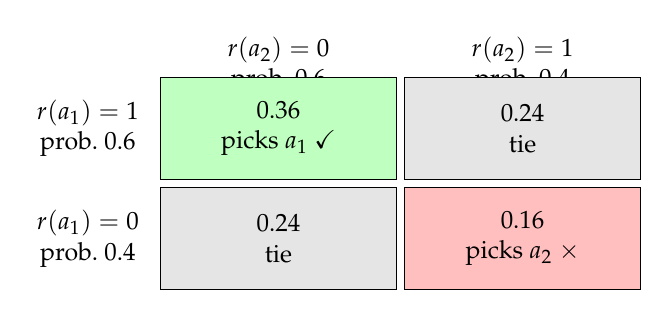
\begin{tikzpicture}[font=\small,every node/.style={align=center}]
  \foreach \i/\l in {0/{$r(a_2)=0$\\ prob.\ $0.6$},1/{$r(a_2)=1$\\ prob.\ $0.4$}}
     \node at (3.1*\i+1.55,2.7) {\l};
  \node[left] at (-0.1,1.9) {$r(a_1)=1$\\ prob.\ $0.6$};
  \node[left] at (-0.1,0.5) {$r(a_1)=0$\\ prob.\ $0.4$};
  \node[draw,fill=green!25,minimum width=3cm,minimum height=1.3cm] at (1.55,1.9) {$0.36$\\ picks $a_1$ \checkmark};
  \node[draw,fill=black!10,minimum width=3cm,minimum height=1.3cm] at (4.65,1.9) {$0.24$\\ tie};
  \node[draw,fill=black!10,minimum width=3cm,minimum height=1.3cm] at (1.55,0.5) {$0.24$\\ tie};
  \node[draw,fill=red!25,minimum width=3cm,minimum height=1.3cm] at (4.65,0.5) {$0.16$\\ picks $a_2$ $\times$};
\end{tikzpicture}
\caption{Outcomes of the first two pulls in the greedy example (probabilities multiply because the arms are independent).}
\end{figure}

\begin{intuition}
Greedy treats one noisy sample as the truth. If ties are broken uniformly, the probability of locking onto
the worse arm is $0.16+0.24=0.40$ (not just the $16\%$ highlighted on the slide), and once committed it loses
$0.2$ per round forever, so the expected regret is about $0.4\times0.2\,T=0.08\,T$: \emph{linear} in $T$.
Any sensible algorithm must keep sampling long enough to be confident.
\end{intuition}

\subsection{Explore \& Commit Algorithm \slides{8}}

\begin{algorithm}[Explore-then-commit, MAB]
Choose an exploration length $N$ per arm (the slide writes $N=T/K$ as a placeholder; it must satisfy $NK\ll T$, and
the optimised value is derived on slide~12).
\begin{enumerate}
  \item \textbf{Explore.} For $k=1,\dots,K$: pull arm $k$ exactly $N$ times and compute the empirical mean
        $\hat\mu_k=\frac1N\sum_{i=1}^N r_i$.
  \item \textbf{Commit.} For $t=NK,\dots,T-1$: pull $\hat I=\argmax_{i\in[K]}\hat\mu_i$.
\end{enumerate}
\end{algorithm}

\subsection{Hoeffding Inequality \slides{9--10}}

To say how wrong $\hat\mu$ can be, we need a confidence interval.

\begin{theorem}[Hoeffding inequality (Lecture~1, Thm.~5)]\label{thm:hoeffding}
Let $X_1,\dots,X_N\in[0,1]$ be i.i.d.\ with mean $\mu$. For every $\delta\in(0,1)$, with probability at least $1-\delta$,
\[
 \Bigl|\tfrac1N\textstyle\sum_{i=1}^N X_i-\mu\Bigr|\;\le\;\sqrt{\frac{\ln(2/\delta)}{2N}} \;=\;O\!\Bigl(\sqrt{\tfrac{\ln(1/\delta)}{N}}\Bigr).
\]
Applying it to all $K$ arms at once with a union bound (replace $\delta$ by $\delta/K$) gives, with probability at least $1-\delta$,
$|\hat\mu_i-\mu_i|\le\sqrt{\ln(2K/\delta)/(2N)}$ \emph{simultaneously} for every arm $i$.
\end{theorem}

\begin{figure}[ht]
\centering
\begin{tikzpicture}[font=\small]
  \begin{scope}
    \civ{0}{2}{1.55}{2}
    \node[left] at (-0.15,4) {$\hat\mu+\sqrt{\ln(1/\delta)/N}$};
    \node[left] at (-0.15,2) {$\hat\mu$};
    \node[left] at (-0.15,0) {$\hat\mu-\sqrt{\ln(1/\delta)/N}$};
    \node[right,green!50!black] at (0.15,1.55) {$\mu$ (unknown, inside the interval w.p.\ $1-\delta$)};
  \end{scope}
  \begin{scope}[xshift=8.2cm]
    \draw[->] (-0.3,-0.6) -- (-0.3,4.4) node[above] {reward};
    \civ{1}{2.1}{1.75}{0.9}  \civ{2.5}{2.7}{2.5}{0.9}  \civ{4}{1.5}{1.8}{0.9}
    \foreach \x/\a in {1/1,2.5/2,4/3} \node[below] at (\x,-0.1) {arm $\a$};
    \draw[dotted] (0.6,3.0) -- (4.4,3.0) (0.6,1.2) -- (4.4,1.2);
    \node[font=\scriptsize,align=center] at (2.5,4.3) {same width $\sqrt{\ln(K/\delta)/N}$ for all arms};
  \end{scope}
\end{tikzpicture}
\caption{Left (slide 9): the confidence interval around one empirical mean; the true mean (green) lies inside with
probability $1-\delta$. Right (slide 10): during commitment, all $K$ intervals hold simultaneously, so the width
contains $\ln(K/\delta)$. Black dots: $\hat\mu_i$ and interval ends.}
\end{figure}

\begin{intuition}
The interval shrinks like $1/\sqrt N$: to halve the uncertainty you need four times the data. With $\delta=0.01$
(``the bound holds with probability 99\%'') and $N=100$ samples, the half-width is
$\sqrt{\ln(200)/200}\approx0.163$; with $N=1000$ it is $\approx0.051$. For $K=10$ arms and $N=100$, the union bound
makes it $\sqrt{\ln(2000)/200}\approx0.195$: the price of ``all arms at once'' is only logarithmic in $K$.
\end{intuition}

\subsection{Regret Calculation \slides{11--12}}

Let $\hat I=\argmax_i\hat\mu_i$ (empirical best arm) and $I^\star=\argmax_i\mu_i$ (best arm).

\begin{theorem}[Regret of explore-then-commit, MAB]\label{thm:ec-mab}
Let $L=\ln(2K/\delta)$ (the slides write $\ln(K/\delta)$, absorbing constants into the $O(\cdot)$) and $1\le NK\le T$. With probability at least $1-\delta$,
\[
 \Reg_T=\Reg_{\mathrm{explore}}+\Reg_{\mathrm{exploit}}\;\le\; NK+2T\sqrt{\frac{L}{N}} .
\]
Choosing $N^\star=\bigl(T\sqrt{L}/K\bigr)^{2/3}$ gives
$\Reg_T\le 3\,T^{2/3}K^{1/3}L^{1/3}=O\bigl(T^{2/3}K^{1/3}\ln^{1/3}(K/\delta)\bigr)$.
\end{theorem}
\begin{proof}
Let $\varepsilon=\sqrt{L/(2N)}$. By Theorem~\ref{thm:hoeffding} all $|\hat\mu_i-\mu_i|\le\varepsilon$ on an event of probability $\ge1-\delta$. On it,
\[
 \mu_{I^\star}\le\hat\mu_{I^\star}+\varepsilon\le\hat\mu_{\hat I}+\varepsilon\le\mu_{\hat I}+2\varepsilon ,
\]
so every committed round costs at most $2\varepsilon$. Exploration lasts $NK$ rounds with per-round regret $\le1$, so
$\Reg_{\mathrm{explore}}\le NK$, and $\Reg_{\mathrm{exploit}}\le(T-NK)\,2\varepsilon\le 2T\sqrt{L/N}$.
For the second claim let $f(N)=NK+2T\sqrt L\,N^{-1/2}$. Then $f'(N)=K-T\sqrt L\,N^{-3/2}$ vanishes at $N^\star=(T\sqrt L/K)^{2/3}$
and $f$ is convex, so this is the minimiser. From $N^{\star3/2}=T\sqrt L/K$ we get $2T\sqrt L\,N^{\star-1/2}=2KN^\star$, hence
$f(N^\star)=3KN^\star=3K^{1/3}T^{2/3}L^{1/3}$ (ignoring rounding of $N^\star$).
\end{proof}

\begin{figure}[ht]
\centering
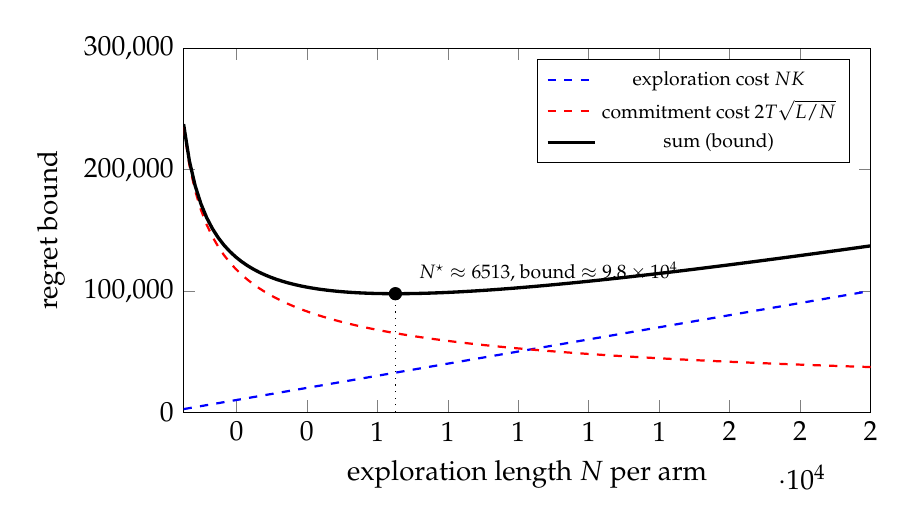
\begin{tikzpicture}
\begin{axis}[width=0.85\linewidth,height=6.2cm,xlabel={exploration length $N$ per arm},ylabel={regret bound},
  xmin=500,xmax=20000,ymin=0,ymax=300000,domain=500:20000,samples=120,no markers,
  legend style={font=\scriptsize,at={(0.97,0.97)},anchor=north east},scaled y ticks=false,
  yticklabel style={/pgf/number format/fixed,/pgf/number format/precision=0},
  xticklabel style={/pgf/number format/fixed,/pgf/number format/precision=0}]
 \addplot[blue,dashed,thick]{5*x};
 \addplot[red,dashed,thick]{2*1000000*sqrt(6.9078/x)};
 \addplot[black,very thick]{5*x+2*1000000*sqrt(6.9078/x)};
 \addlegendentry{exploration cost $NK$}
 \addlegendentry{commitment cost $2T\sqrt{L/N}$}
 \addlegendentry{sum (bound)}
 \addplot[only marks,mark=*,mark size=2.2pt,black,forget plot] coordinates {(6513,97700)};
 \draw[dotted] (axis cs:6513,0) -- (axis cs:6513,97700);
 \node[anchor=south west,font=\scriptsize] at (axis cs:6900,100000) {$N^\star\approx 6513$, bound $\approx 9.8\times10^4$};
\end{axis}
\end{tikzpicture}
\caption{The explore/exploit trade-off inside Theorem~\ref{thm:ec-mab} for $T=10^6$, $K=5$, $\delta=0.01$ ($L\approx6.91$):
more exploration costs linearly, but shrinks the commitment error like $1/\sqrt N$.}
\end{figure}

\begin{intuition}
Too little exploration makes you commit to the wrong arm; too much wastes rounds on bad arms. The optimum balances the
two curves (at $N^\star$ the commitment term is exactly twice the exploration term). Numerically, for $T=10^6$,
$K=5$, $\delta=0.01$: $N^\star\approx6{,}513$ pulls per arm, i.e.\ $\approx32{,}600$ exploration rounds (3.3\% of $T$), and
a regret bound of $\approx9.8\times10^4$, about $9.8\%$ of the maximum possible. Dividing by $T$, the \emph{average}
regret per round decays like $T^{-1/3}$, i.e.\ it ``approaches~0 as $T\to\infty$'' (slide~12), but slowly.
\end{intuition}

\subsection{Regret Decaying \slides{13}}

The $T^{2/3}$ rate of explore-then-commit is ``kind of slow''. The slide asks for something like $O(\sqrt T)$ and states that
$\sqrt T$ is the best possible: it is a \emph{lower bound}, no algorithm can do better in the worst case
(the standard minimax bound is $\Omega(\sqrt{KT})$; it is quoted, not proved, in the lecture). So we look for a new algorithm.

\begin{figure}[ht]
\centering
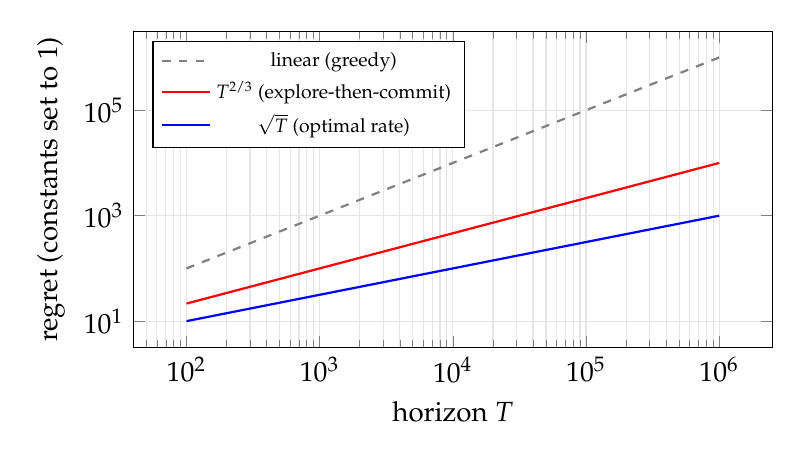
\begin{tikzpicture}
\begin{loglogaxis}[width=0.8\linewidth,height=5.6cm,xlabel={horizon $T$},ylabel={regret (constants set to 1)},
  domain=1e2:1e6,samples=40,no markers,legend style={font=\scriptsize,at={(0.03,0.97)},anchor=north west},grid=both,
  grid style={black!10}]
 \addplot[gray,dashed,thick]{x};
 \addplot[red,thick]{x^(2/3)};
 \addplot[blue,thick]{x^(1/2)};
 \addlegendentry{linear (greedy)}
 \addlegendentry{$T^{2/3}$ (explore-then-commit)}
 \addlegendentry{$\sqrt T$ (optimal rate)}
\end{loglogaxis}
\end{tikzpicture}
\caption{Growth rates compared (slide 13 describes them in words). On a log--log plot a rate $T^\alpha$ is a line of slope~$\alpha$.}
\end{figure}

\begin{intuition}
For $T=10^6$: $\sqrt T=10^3$ versus $T^{2/3}=10^4$. A tenfold gap, i.e.\ per-round regret $0.1\%$ versus $1\%$ (with all constants set to~1).
\end{intuition}

\subsection{Statistics to Maintain \& Confidence \slides{14}}

To compute confidence bounds \emph{while} learning we keep, for each arm $i$ at time $t$:
\[
 N_t(i)=\sum_{\tau=0}^{t-1}\ind\{I_\tau=i\},\qquad
 \hat\mu_t(i)=\frac{1}{N_t(i)}\sum_{\tau=0}^{t-1}\ind\{I_\tau=i\}\,r_\tau ,
\]
and, with probability $1-\delta$ (simultaneously for all arms and all times),
\[
 |\hat\mu_t(i)-\mu_i|\le\sqrt{\frac{\ln(KT/\delta)}{N_t(i)}} .
\]

\begin{intuition}
Unlike explore-then-commit, arms now have \emph{different} sample sizes, so each arm gets its \emph{own} interval width.
The $KT$ inside the logarithm is a union bound over every (arm, time) pair, because the algorithm will consult these bounds at every round.
\end{intuition}

\subsection{Optimism in the Face of Uncertainty \slides{15}}

Pick the arm with the highest \emph{upper} confidence bound (the top of its interval).

\begin{figure}[ht]
\centering
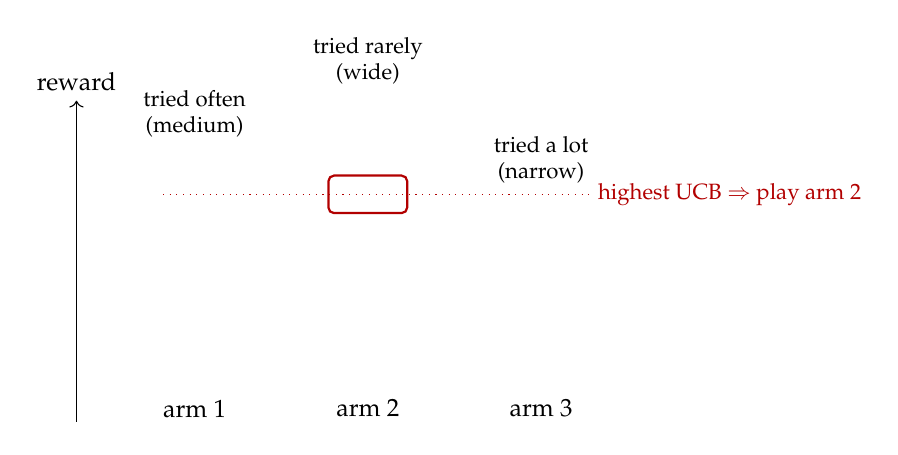
\begin{tikzpicture}[font=\small,y=3.4cm]
  \civ{1}{0.55}{0.5}{0.2}  \civ{3.2}{0.5}{0.6}{0.35}  \civ{5.4}{0.6}{0.58}{0.1}
  \foreach \x/\a in {1/1,3.2/2,5.4/3} \node[below=3pt] at (\x,0.15) {arm $\a$};
  \draw[red!70!black,thick,rounded corners=2pt] (2.7,0.78) rectangle (3.7,0.92);
  \draw[dotted,red!70!black] (0.6,0.85) -- (6.0,0.85);
  \node[red!70!black,right,font=\footnotesize] at (6.0,0.85) {highest UCB $\Rightarrow$ play arm 2};
  \node[font=\footnotesize,align=center] at (1,1.15) {tried often\\(medium)};
  \node[font=\footnotesize,align=center] at (3.2,1.35) {tried rarely\\(wide)};
  \node[font=\footnotesize,align=center] at (5.4,0.98) {tried a lot\\(narrow)};
  \draw[->] (-0.5,0.0) -- (-0.5,1.2) node[above] {reward};
\end{tikzpicture}
\caption{Optimism (slide 15). Arm~2 has a \emph{lower} empirical mean than arm~3, but its wide interval (few pulls) gives the highest upper bound, so UCB explores it.
Green dots: true means.}
\end{figure}

\subsection{UCB Algorithm \slides{16}}

\begin{algorithm}[UCB]\label{alg:ucb}
Pull each arm once (first $K$ rounds). For $t=K,\dots,T-1$:
\begin{enumerate}
  \item pick $\displaystyle I_t=\argmax_{i\in[K]}\Bigl(\hat\mu_t(i)+\sqrt{\tfrac{\ln(KT/\delta)}{N_t(i)}}\Bigr)$;
  \item observe the reward and update $N_t,\hat\mu_t$.
\end{enumerate}
The square-root \emph{reward bonus} is large for arms not tried many times, which drives exploration.
\end{algorithm}

\begin{intuition}
UCB acts as if each arm were as good as it \emph{could plausibly be}. Under-sampled arms get an inflated score and are tried;
if the optimism was unjustified, the empirical mean drops and $N_t(i)$ grows, so the bonus shrinks and the arm is abandoned.
Nothing is hard-coded about \emph{when} to stop exploring: the schedule emerges from the data. Exploration and exploitation are fused into one rule.
\end{intuition}

\subsection{UCB Algorithm: Regret \slides{17}}

\begin{theorem}[Regret of UCB (Lecture~1)]\label{thm:ucb}
Let $L'=\ln(2KT/\delta)$. With probability at least $1-\delta$, UCB satisfies
$\Reg_T\le K+4\sqrt{KT\,L'}=\widetilde O(\sqrt{KT})$.
\end{theorem}
\begin{proof}
On the event that all intervals hold, write $w_t=\sqrt{L'/N_t(I_t)}$. Then
\[
 \mu^\star\le \hat\mu_t(I^\star)+\sqrt{\tfrac{L'}{N_t(I^\star)}}\le \hat\mu_t(I_t)+w_t\le\mu_{I_t}+2w_t,
\]
so the per-round regret is $\mu^\star-\mu_{I_t}\le 2w_t$ (the first inequality is validity of the interval for $I^\star$, the second is the UCB rule, the third is validity for $I_t$). Summing over $t\ge K$,
\[
 \sum_{t=K}^{T-1}\frac1{\sqrt{N_t(I_t)}}=\sum_{i}\sum_{n=1}^{N_T(i)-1}\frac1{\sqrt n}\le\sum_i 2\sqrt{N_T(i)}\le 2\sqrt{K\textstyle\sum_iN_T(i)}\le2\sqrt{KT},
\]
by $\sum_{n\le m}n^{-1/2}\le2\sqrt m$ and Cauchy--Schwarz. The first $K$ rounds cost at most $K$. Hence $\Reg_T\le K+2\sqrt{L'}\cdot2\sqrt{KT}$.
\end{proof}

\begin{intuition}
Each arm contributes $\sum_{n\le N}1/\sqrt n\approx2\sqrt N$ to the regret sum, and the total number of pulls is capped at $T$; the worst case is spreading
pulls evenly, which yields $\sqrt{KT}$. For $K=5$, $T=10^6$ the \emph{rate} is $\approx\sqrt{5\cdot10^6}\approx2.2\times10^3$ (times $\sqrt{\ln}$ and a constant),
versus the $T^{2/3}$ rate of explore-then-commit which is of order $10^4$. (The slide cites an external note for details, \url{https://wensun.github.io/CS4789_data/UCB_note_new.pdf}.)
\end{intuition}
% =====================================================================
\section{From Multi-Armed to Contextual Bandits \slides{19--24}}

\subsection{From Multi-Armed to Contextual Bandits \slides{19--20}}

A multi-armed bandit is \emph{stateless}: an action leads to a reward. A \textbf{contextual bandit} adds a context (state)
that is observed before acting and that influences which action is best.

\begin{figure}[ht]
\centering
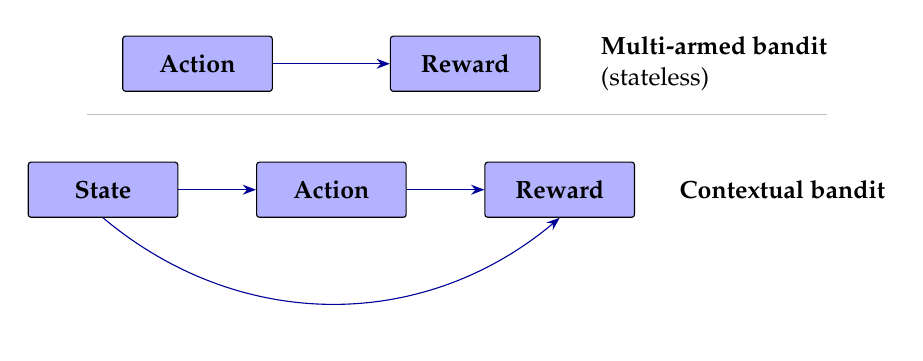
\begin{tikzpicture}[>=Stealth,font=\small,
  blk/.style={draw,fill=blue!30,rounded corners=1pt,minimum width=1.9cm,minimum height=0.7cm,font=\small\bfseries}]
  \node[blk] (a1) at (0,1.6) {Action};  \node[blk] (r1) at (3.4,1.6) {Reward};
  \draw[->,blue!60!black] (a1) -- (r1);
  \node[align=left,anchor=west] at (5.0,1.6) {\textbf{Multi-armed bandit}\\ (stateless)};
  \draw[black!25] (-1.4,0.95) -- (8,0.95);
  \node[blk] (s2) at (-1.2,0) {State};  \node[blk] (a2) at (1.7,0) {Action};  \node[blk] (r2) at (4.6,0) {Reward};
  \draw[->,blue!60!black] (s2) -- (a2);  \draw[->,blue!60!black] (a2) -- (r2);
  \draw[->,blue!60!black] (s2.south) to[bend right=40] (r2.south);
  \node[align=left,anchor=west] at (6.0,0) {\textbf{Contextual bandit}};
\end{tikzpicture}
\caption{Slides 19--20 redrawn. In a contextual bandit the reward depends on the \emph{state/context and the action}
(the curved arrow).}
\end{figure}

\subsection{Contextual Bandits: Interaction \slides{21--23}}

\begin{definition}[Contextual bandit]\label{def:cb}
A contextual bandit is a distribution $\rho$ over a context set $\calX$ together with a mean-reward function
$r:\calX\times\calA\to[0,1]$, where $|\calA|=K$. For $t=0,1,\dots,T-1$:
\begin{enumerate}
 \item a context $x_t\sim\rho$ is drawn i.i.d.\ and \emph{revealed};
 \item the learner picks $a_t\in\calA$, possibly at random, using $x_t$ and the history;
 \item a reward $r_t$ with $\E[r_t\mid x_t,a_t]=r(x_t,a_t)$ is revealed, and nothing is revealed about the other $K-1$ actions.
\end{enumerate}
\end{definition}

\begin{remark}
For simplicity the slides (slide~22) assume \emph{deterministic} rewards $r_t=r(x_t,a_t)$, ``as the context is the challenge here'';
the companion note stresses that every result below holds with noisy rewards too (the proof of Lemma~\ref{lem:ips}
conditions on the noise).
\end{remark}

\begin{figure}[ht]
\centering
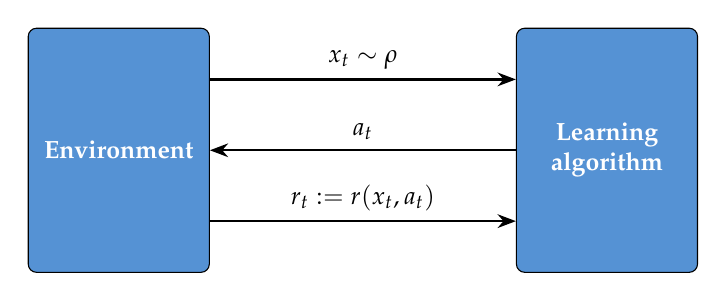
\begin{tikzpicture}[>=Stealth,font=\small,
  box/.style={draw,fill=cyan!55!blue!70,rounded corners=3pt,minimum width=2.3cm,minimum height=3.1cm,text=white,align=center,font=\small\bfseries}]
  \node[box] (env) at (0,0) {Environment};
  \node[box] (alg) at (6.2,0) {Learning\\algorithm};
  \draw[->,thick] ($(env.east)+(0,0.9)$) -- node[above] {$x_t\sim\rho$} ($(alg.west)+(0,0.9)$);
  \draw[->,thick] ($(alg.west)+(0,0)$) -- node[above] {$a_t$} ($(env.east)+(0,0)$);
  \draw[->,thick] ($(env.east)+(0,-0.9)$) -- node[above] {$r_t:=r(x_t,a_t)$} ($(alg.west)+(0,-0.9)$);
\end{tikzpicture}
\caption{The interaction protocol (slide 23). After the reward, a new round starts: contexts are \emph{not} influenced by past actions, they are sampled i.i.d.}
\end{figure}

\begin{intuition}
The i.i.d.\ context is what separates a contextual bandit from a full MDP: your action affects your \emph{reward} today but not the \emph{state}
you will see tomorrow, so there are no long-term consequences to plan around. It is a bandit with side information. The difficulty that remains is that
the best action depends on the context, and you only see the reward of the action you actually took.
\end{intuition}

\subsection{Contextual Bandits: Example \slides{24}}

A major application is \textbf{recommendation systems}: the \emph{context} is user information (age, height, weight, job, \dots), the \emph{arms} are items to recommend
(news, movies, \dots), and each arm has a click-through rate (0/1 reward) that we want to maximise. The question: how do we decide which item to propose next \emph{in a personalised way}?

\begin{example}\label{ex:reco}
Two equally frequent user types and two items, with click-through rates

\smallskip
\begin{center}
\begin{tabular}{lcc}\toprule
 & news & movies\\\midrule
 younger users & $0.10$ & $0.30$\\ older users & $0.35$ & $0.15$\\\bottomrule
\end{tabular}
\end{center}
A context-blind bandit sees an average CTR of $0.225$ for both items and earns $0.225$ per round at best, whereas the personalised rule
(movies for younger, news for older) earns $\tfrac12(0.30+0.35)=0.325$.
\end{example}

\begin{intuition}
Ignoring context averages away exactly the structure that matters. But learning one separate bandit per context is hopeless when contexts are
many or continuous (every user is unique). The remedy, developed next, is to learn a \emph{policy} from a restricted class $\Pi$ that generalises across contexts.
\end{intuition}

% =====================================================================
\section{Policy \slides{25}}

\begin{definition}[Policy]\label{def:policy}
A policy $\pi$ is a mapping from (all) states/contexts to actions that determines how the agent selects actions. It can be
\emph{deterministic}, $a=\pi(x)$, or \emph{stochastic}, $\pi(a\mid x)$ (equivalently $a\sim\pi(\cdot\mid x)$). Given a class $\Pi$ of policies, the
\emph{value} of $\pi$ is its expected reward, $V(\pi)=\E_{x\sim\rho}\bigl[r(x,\pi(x))\bigr]$.
\end{definition}

\begin{intuition}
A policy is a rulebook: ``if the user looks like this, show that''. For a finite context set $\calX$ with $K$ actions there are $K^{|\calX|}$ deterministic policies:
with $|\calX|=10$ and $K=3$ that is $3^{10}=59{,}049$, huge, but its \emph{logarithm} is only $10\ln3\approx10.99$. It is this logarithm, $\ln|\Pi|$, that will govern the regret.
\end{intuition}

% =====================================================================
\section{Contextual Bandits: Regret \slides{26}}

The optimal policy in the class is $\pi^\star=\argmax_{\pi\in\Pi}\E_{x\sim\rho}\,r(x,\pi(x))=\argmax_{\pi\in\Pi}V(\pi)$.
At every round $a_t=\pi_t(x_t)$ is selected and a reward received.

\begin{definition}[Contextual regret]\label{def:reg}
\[
 \mathrm{Reg}(T)\;=\;T\,V(\pi^\star)-\sum_{t=0}^{T-1}V(\pi_t)
 \;=\;T\,\E_{x\sim\rho}\bigl[r(x,\pi^\star(x))\bigr]-\sum_{t=0}^{T-1}\E_{x\sim\rho}\bigl[r(x,\pi_t(x))\bigr],
\]
where $\pi_t$ is the policy the learner is using at round $t$ (note: \emph{it changes at every iteration}).
\end{definition}

\begin{intuition}
The first term is the total expected reward if we always used the best policy; the second is what our sequence of learned policies earns.
If $\calX$ is a single context, $V(\pi)=r(a)$ and this is exactly the multi-armed regret of Section~1. In the recommendation example the
best policy earns $0.325$ per round, so a context-blind learner has regret at least $(0.325-0.225)T=0.1\,T$, linear in $T$.
\end{intuition}

% =====================================================================
\section{Explore \& Commit Algorithm \slides{27--31}}

\subsection{The algorithm \slides{27}}

\begin{algorithm}[Explore-then-commit for contextual bandits]\label{alg:ec}
Input: horizon $T$, policy class $\Pi$, exploration budget $N$.
\begin{enumerate}
 \item \textbf{Explore.} For $t=0,\dots,N-1$: observe $x_t\sim\rho$, draw $a_t\sim\Unif(\calA)$, observe $r_t=r(x_t,a_t)$, and build for $x_t$ an
       \emph{unbiased estimate} $\rh_t$ of the reward vector $\bigl(r(x_t,a)\bigr)_{a\in\calA}$.
 \item \textbf{Fit.} Compute the policy $\displaystyle\hat\pi\in\argmax_{\pi\in\Pi}\sum_{t=0}^{N-1}\rh_t[\pi(x_t)]$.
 \item \textbf{Commit.} For $t=N,\dots,T-1$: observe $x_t\sim\rho$ and play $a_t=\hat\pi(x_t)$.
\end{enumerate}
\end{algorithm}

The missing ingredient is the unbiased estimate $\rh_t$: we only observe the reward of \emph{one} action.

\subsection{Unbiased estimates: inverse propensity scoring \slides{27--29}}

An estimator $\hat\theta$ is \emph{unbiased} if $\E[\hat\theta]=\theta$, i.e.\ $\mathrm{bias}(\hat\theta)=\E[\hat\theta]-\theta=0$ (it is centred on the true value).
The goal here: $\E_{a_t\sim p}\bigl[\rh_t[a]\bigr]=r(x_t,a)$ for all $a$.

\begin{definition}[Inverse propensity scoring (IPS)]\label{def:ips}
Suppose that at round $t$ the action was drawn from a \emph{known} distribution $p_t$ with $p_t(a)>0$ for all $a$. The IPS reward vector is
\[
 \rh_t[a]=\frac{r_t\,\ind[a_t=a]}{p_t(a)},\qquad a\in\calA,
\]
i.e.\ the vector with a single non-zero entry $r_t/p_t(a_t)$ at the played action. Under uniform exploration, $p_t(a)=1/K$ and
$\rh_t[a]=\bigl\{K r_t$ if $a=a_t$, $0$ otherwise$\bigr\}$ (slide 29: ``$r_t/(1/|\calA|)$'').
\end{definition}

\begin{lemma}[IPS is unbiased]\label{lem:ips}
For every context $x_t$ and every action $a$, $\E_{a_t\sim p_t}\bigl[\rh_t[a]\mid x_t\bigr]=r(x_t,a)$. Consequently
$\E\bigl[\rh_t[\pi(x_t)]\bigr]=V(\pi)$ for every policy $\pi$.
\end{lemma}
\begin{proof}
Condition on $x_t$ and take the expectation over $a_t\sim p_t$ and the reward noise:
\[
 \E\!\left[\frac{r_t\,\ind[a_t=a]}{p_t(a)}\right]=\sum_{a'\in\calA}p_t(a')\,\frac{\E[r_t\mid x_t,a']\,\ind[a'=a]}{p_t(a)}
 =p_t(a)\,\frac{r(x_t,a)}{p_t(a)}=r(x_t,a).
\]
Averaging over $x_t\sim\rho$ gives $\E[\rh_t[\pi(x_t)]]=V(\pi)$.
\end{proof}

\begin{intuition}
The division by $p_t(a)$ ``removes the asymmetry due to sampling'' (slide 28): an action played half as often has its rewards counted twice as heavily,
exactly like survey weights that up-weight under-sampled groups. A concrete check with $K=2$, uniform exploration and $r(x,2)=0.8$: whenever arm~2 is played
(half the time) we record $\rh=(0,\,1.6)$, otherwise $(\cdot,\,0)$, so the average is $\tfrac12\cdot1.6+\tfrac12\cdot0=0.8$. The estimator is unbiased
but \emph{noisy}: a single observation is either $0$ or $Kr_t$, far from the true mean (made precise in Lemma~\ref{lem:range}, Appendix~\ref{app:supp}).
Importantly, $\rh_t$ is defined for \emph{all} actions even though only one is observed, which is what lets us evaluate policies that would have acted differently.
\end{intuition}

\subsection{Fitting a policy \slides{27}}

Step~2 of Algorithm~\ref{alg:ec} maximises the \emph{counterfactual value estimate}
$\hat V(\pi)=\frac1N\sum_{t<N}\rh_t[\pi(x_t)]$ over $\Pi$. By Lemma~\ref{lem:ips} each summand has mean $V(\pi)$, so $\hat V(\pi)$ estimates $V(\pi)$ for \emph{every} $\pi\in\Pi$ from the \emph{same} exploration data.

\begin{intuition}
Under uniform exploration, a round only ``counts'' for policy $\pi$ if $\pi(x_t)$ happens to equal the randomly played $a_t$ (probability $1/K$), and then it counts with weight $K r_t$.
In the toy problem below (two contexts, two arms) the four deterministic policies have values
$V(a_1,a_1)=0.525$, $V(a_1,a_2)=0.675$, $V(a_2,a_1)=0.425$, $V(a_2,a_2)=0.575$ (red~$\to$~first entry, blue~$\to$~second), so $\pi^\star=(a_1,a_2)$.
Because $\Pi$ here contains \emph{all} context-to-action maps, the maximisation splits into one independent argmax per context; for a restricted class (e.g.\ linear policies) it does not.
\end{intuition}

\subsection{Simulation \slides{30}}

Slide~30 shows an animation of the explore phase: a timeline of contexts (red/blue) and, per context, the running estimates of each arm's reward. Here is an original static version.

\begin{figure}[ht]
\centering
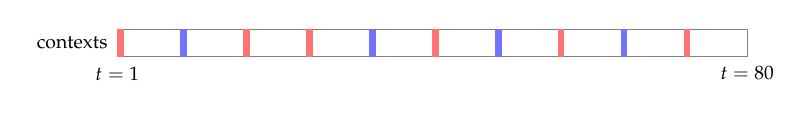
\begin{tikzpicture}
  \draw[black!50] (0,0) rectangle (8,0.35);
  \foreach \x/\c in {0/red!55,0.1/blue!55,0.2/red!55,0.3/red!55,0.4/blue!55,0.5/red!55,0.6/blue!55,0.7/red!55,0.8/blue!55,0.9/red!55} {
    \fill[\c] (8*\x,0) rectangle (8*\x+0.08,0.35);
  }
  \node[left,font=\scriptsize] at (0,0.175) {contexts};
  \node[below,font=\scriptsize] at (0,0) {$t=1$}; \node[below,font=\scriptsize] at (8,0) {$t=80$};
\end{tikzpicture}\\[4pt]
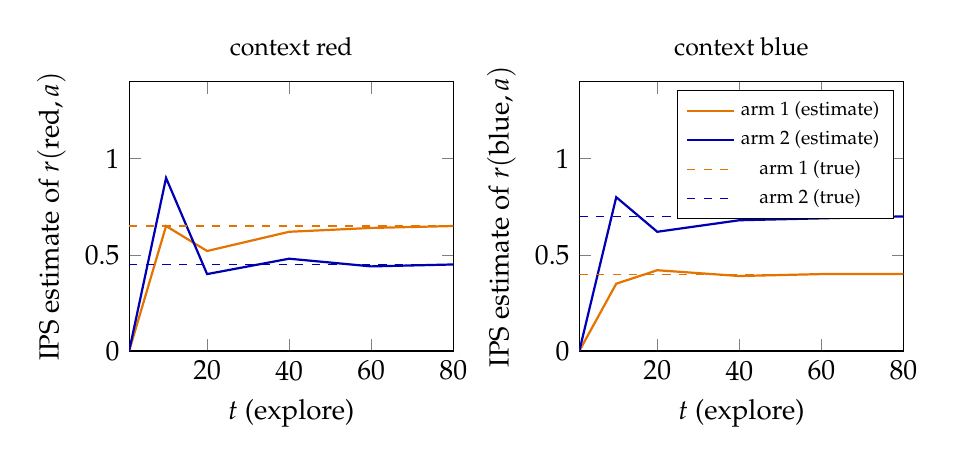
\begin{tikzpicture}
\begin{groupplot}[group style={group size=2 by 1,horizontal sep=1.6cm},width=0.47\linewidth,height=5cm,
  xmin=1,xmax=80,ymin=0,ymax=1.4,xlabel={$t$ (explore)},no markers,title style={font=\small}]
 \nextgroupplot[title={context red},ylabel={IPS estimate of $r(\text{red},a)$}]
  \addplot[orange!90!black,thick] coordinates {(1,0.00) (10,0.65) (20,0.52) (40,0.62) (60,0.64) (80,0.65)};
  \addplot[blue!70!black,thick] coordinates {(1,0.00) (10,0.90) (20,0.40) (40,0.48) (60,0.44) (80,0.45)};
  \addplot[orange!90!black,dashed] coordinates {(1,0.65) (80,0.65)};
  \addplot[blue!70!black,dashed] coordinates {(1,0.45) (80,0.45)};
 \nextgroupplot[title={context blue},ylabel={IPS estimate of $r(\text{blue},a)$},legend style={font=\scriptsize,at={(0.97,0.97)},anchor=north east}]
  \addplot[orange!90!black,thick] coordinates {(1,0.00) (10,0.35) (20,0.42) (40,0.39) (60,0.40) (80,0.40)};
  \addplot[blue!70!black,thick] coordinates {(1,0.00) (10,0.80) (20,0.62) (40,0.68) (60,0.69) (80,0.70)};
  \addplot[orange!90!black,dashed] coordinates {(1,0.40) (80,0.40)};
  \addplot[blue!70!black,dashed] coordinates {(1,0.70) (80,0.70)};
  \addlegendentry{arm 1 (estimate)}
 \addlegendentry{arm 2 (estimate)}
 \addlegendentry{arm 1 (true)}
 \addlegendentry{arm 2 (true)}
\end{groupplot}
\end{tikzpicture}
\caption{Toy simulation of the explore phase (seeded; $N=80$, uniform exploration, two equally likely contexts, deterministic rewards
$r(\text{red},\cdot)=(0.65,0.45)$, $r(\text{blue},\cdot)=(0.40,0.70)$). Solid: per-context IPS averages; dashed: true values. They are noisy at first but
settle on the correct ordering, so $\hat\pi=\pi^\star$ in this run (about $81\%$ of 2000 seeds at $N=80$).}
\end{figure}

\subsection{Explore \& Commit Algorithm: Regret \slides{31}}

The slide states that the regret ``also depends on the size of the class of policies''. Here is the precise statement.

\begin{theorem}[Regret of contextual explore-then-commit]\label{thm:cec}
Let $\Pi$ be finite and run Algorithm~\ref{alg:ec} with $1\le N\le T$. With probability at least $1-\delta$,
\[
 \mathrm{Reg}(T)\;\le\;N+TK\sqrt{\frac{2\ln(2|\Pi|/\delta)}{N}},
\]
and choosing $N$ to minimise the right-hand side gives
\[
 \mathrm{Reg}(T)\;\le\;3\cdot2^{-1/3}\,T^{2/3}K^{2/3}\ln^{1/3}\!\Bigl(\frac{2|\Pi|}{\delta}\Bigr).
\]
\end{theorem}
\begin{proof}
Write $\hat V(\pi)=\frac1N\sum_{t<N}\rh_t[\pi(x_t)]$. By Lemma~\ref{lem:ips} the summands are i.i.d.\ with mean $V(\pi)$ and by Lemma~\ref{lem:range} (Appendix~\ref{app:supp})
they lie in $[0,K]$. Hoeffding's inequality (Theorem~\ref{thm:hoeffding}, rescaled by $K$) gives, for one fixed $\pi$ and any $\delta'\in(0,1)$,
\[
 \Prob\Bigl(|\hat V(\pi)-V(\pi)|>K\sqrt{\ln(2/\delta')/(2N)}\Bigr)\le\delta'.
\]
Take $\delta'=\delta/|\Pi|$ and a union bound over the $|\Pi|$ policies: with probability at least $1-\delta$, every $\pi\in\Pi$ satisfies
$|\hat V(\pi)-V(\pi)|\le\varepsilon$ with $\varepsilon=K\sqrt{\ln(2|\Pi|/\delta)/(2N)}$.
On that event, the same three-step chain as in Theorem~\ref{thm:ec-mab} applies to $\hat\pi$, which maximises $\hat V$:
\[
 V(\pi^\star)\le\hat V(\pi^\star)+\varepsilon\le\hat V(\hat\pi)+\varepsilon\le V(\hat\pi)+2\varepsilon .
\]
Exploration contributes at most $N$ (each round's regret is at most $1$); commitment contributes at most $(T-N)\cdot2\varepsilon\le2T\varepsilon$. Adding them gives the first display.

For the second, set $c=\sqrt{2\ln(2|\Pi|/\delta)}$, so the bound reads $f(N)=N+TKc\,N^{-1/2}$. As in the MAB case, $f$ is convex and
$f'(N)=1-\tfrac12TKc\,N^{-3/2}$ vanishes at $N^\star=(TKc/2)^{2/3}$. Writing $u=(TKc/2)^{1/3}$ gives $f(N^\star)=u^2+2u^2=3(TKc/2)^{2/3}$, and substituting
$c^{2/3}=2^{1/3}\ln^{1/3}(2|\Pi|/\delta)$ gives the claim.
\end{proof}

\begin{intuition}
It is the same trade-off as in the MAB: exploring costs $N$ in regret; each extra sample sharpens \emph{all} policy estimates simultaneously, and the union bound over policies only
costs a $\ln|\Pi|$ factor inside the square root. Numerically, for $|\Pi|=10^6$, $K=3$, $\delta=0.05$, $T=10^6$: $\ln(2|\Pi|/\delta)\approx17.5$,
the optimal exploration length is $N^\star\approx4.3\times10^4$ rounds ($4.3\%$ of $T$) and the bound is $\approx1.29\times10^5$ ($12.9\%$ of $T$).
Making the class a million times richer, from $|\Pi|=10^6$ to $10^{12}$, multiplies the bound only by $(3.15/2.60)\approx1.21$ (the factor $\ln^{1/3}(2|\Pi|/\delta)$ goes $2.02\to2.60\to3.15$ for $|\Pi|=10^2,10^6,10^{12}$).
The price of context is thus \emph{logarithmic in the number of policies} but, because uniform exploration wastes a factor $K$ per observation, it grows with $K$.
\end{intuition}

\begin{remark}[On the exponent of $K$]
Slide~31 prints the bound as $O\bigl(T^{2/3}K^{1/3}\ln^{1/3}(|\Pi|)\bigr)$, while the proof above (which only uses the \emph{range} $[0,K]$ of the IPS terms) yields $K^{2/3}$.
The $K^{1/3}$ form is the known sharper rate: using the \emph{variance} bound of Lemma~\ref{lem:range} with Bernstein's inequality instead of Hoeffding's gives
deviations of order $\sqrt{K\ln(|\Pi|/\delta)/N}$ and hence $T^{2/3}K^{1/3}\ln^{1/3}(|\Pi|/\delta)$ plus a lower-order term. This refinement is a standard fact but is
\emph{not} proved in the companion note, so the theorem is stated with the exponent that is actually proved.
\end{remark}
% =====================================================================
\section{\texorpdfstring{$\epsilon$}{epsilon}-Greedy \slides{32--35}}

Instead of fixing a threshold for exploring and then committing, we can \emph{interleave} exploration and exploitation.

\begin{algorithm}[$\epsilon$-greedy for contextual bandits]\label{alg:eg}
For $t=0,1,\dots,T-1$:
\begin{enumerate}
 \item observe $x_t\sim\rho$;
 \item draw $a_t\sim p_t=(1-\epsilon_t)\,\delta\bigl(\pi^t(x_t)\bigr)+\epsilon_t\,\Unif(\calA)$;
 \item observe $r_t$ and form the IPS vector $\rh_t$ using the propensity $p_t(a_t)$ \emph{actually used};
 \item update the policy: $\pi^{t+1}\in\argmax_{\pi\in\Pi}\sum_{i\le t}\rh_i[\pi(x_i)]$.
\end{enumerate}
Gradually \textbf{decay} $\epsilon_t$ towards zero (slide 34, ``Step 3'').
\end{algorithm}

Here $\delta(\pi^t(x_t))$ is the Dirac delta placing all the mass on the action $\pi^t(x_t)$, so explicitly
$p_t(a)=(1-\epsilon_t)\ind[a=\pi^t(x_t)]+\epsilon_t/K$. The two extremes are $\epsilon=0$ (pure exploitation) and $\epsilon=1$ (uniform exploration).
Since $p_t(a)\ge\epsilon_t/K>0$, IPS is well defined, and Lemma~\ref{lem:ips} applies at every round (it only needs $p_t$ to be known, and $p_t$ may change with $t$).

\begin{figure}[ht]
\centering
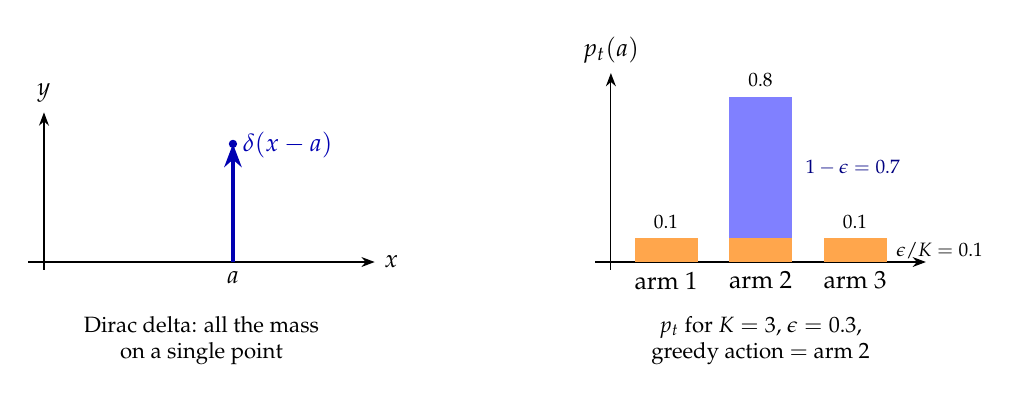
\begin{tikzpicture}[>=Stealth,font=\small]
 \begin{scope}
  \draw[->] (-0.2,0) -- (4.2,0) node[right] {$x$}; \draw[->] (0,-0.1) -- (0,1.9) node[above] {$y$};
  \draw[->,very thick,blue!70!black] (2.4,0) -- (2.4,1.5); \fill[blue!70!black] (2.4,1.5) circle (1.5pt);
  \node[blue!70!black,above right] at (2.4,1.2) {$\delta(x-a)$}; \node[below] at (2.4,0) {$a$};
  \node[align=center,font=\footnotesize] at (2,-1.0) {Dirac delta: all the mass\\on a single point};
 \end{scope}
 \begin{scope}[xshift=7.2cm]
  \draw[->] (-0.2,0) -- (4.0,0); \draw[->] (0,-0.1) -- (0,2.4) node[above] {$p_t(a)$};
  \foreach \x/\n in {0.7/1,1.9/2,3.1/3}{\node[below] at (\x,0) {arm \n};}
  \foreach \x in {0.7,1.9,3.1}{\fill[orange!70] (\x-0.4,0) rectangle (\x+0.4,0.3);}
  \fill[blue!50] (1.9-0.4,0.3) rectangle (1.9+0.4,2.1);
  \node[right,font=\scriptsize] at (3.5,0.15) {$\epsilon/K=0.1$};
  \node[right,font=\scriptsize,blue!50!black] at (2.35,1.2) {$1-\epsilon=0.7$};
  \node[above,font=\scriptsize] at (1.9,2.1) {$0.8$};
  \node[above,font=\scriptsize] at (0.7,0.3) {$0.1$}; \node[above,font=\scriptsize] at (3.1,0.3) {$0.1$};
  \node[align=center,font=\footnotesize] at (1.9,-1.0) {$p_t$ for $K=3$, $\epsilon=0.3$,\\greedy action $=$ arm 2};
 \end{scope}
\end{tikzpicture}
\caption{Left (slide 33): the Dirac delta used in $p_t$. Right: the resulting mixture: every arm gets a floor $\epsilon/K$ of exploration probability and the greedy arm additionally gets $1-\epsilon$.}
\end{figure}

\begin{intuition}
$\epsilon_t$ is a dial between ``trust what I have learned'' and ``roll a die''. The floor $\epsilon_t/K$ is what guarantees every action keeps being sampled so
that IPS stays valid. The dial must be turned down \emph{gradually}: from $r_t\le1$ and $p_t(a)\ge\epsilon_t/K$ we get $0\le\rh_t[a]\le K/\epsilon_t$, so if $\epsilon_t$
collapses, the estimates of rarely played actions become extremely noisy (e.g.\ $\epsilon_t=0.01$, $K=3$ allows values up to $300$). Note that, unlike
explore-then-commit, learning never stops, so the policy keeps adapting. (Neither the slides nor the companion note state a regret bound for $\epsilon$-greedy;
slide 35 only shows a simulation.)
\end{intuition}

\begin{figure}[H]
	\centering
	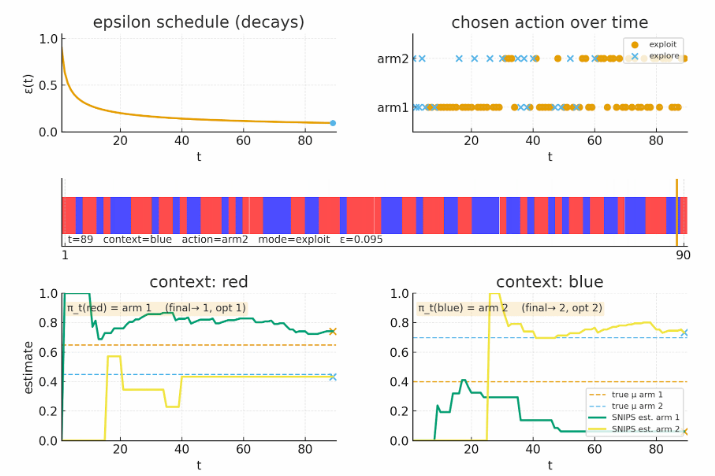
\includegraphics[width=1.0\linewidth]{1790925011807.png}
	\caption{Toy simulation of $\epsilon$-greedy (seeded, $T=90$): early on most rounds are exploratory (open red circles); as $\epsilon_t$ decays the learner mostly exploits its current policy, which here becomes
$\pi=(\text{red}\to\text{arm 1},\ \text{blue}\to\text{arm 2})=\pi^\star$ (27 of the 90 rounds were exploratory). This ends optimal in about $71\%$ of 1000 seeds at $t=90$, so individual runs vary; same colours and dashed true values as the earlier figure.}\label{fig:1790925011807}
\end{figure}




\section{Real World Example \slides{36}}

Slide 36 points to a production use of contextual-bandit algorithms: Microsoft's \emph{Azure Personalizer}
(\url{https://azure.microsoft.com/en-us/products/cognitive-services/personalizer/}), which the slide notes is \emph{going out of service in October 2026}
(the slide shows a screenshot of the product page, not reproduced here).

\begin{intuition}
Personalising content maps one-to-one onto the model of this lecture: the context is the user/page features, the actions are the candidate items, and the reward is a click or
other feedback. Each shown item produces feedback for \emph{that} item only, which is why IPS-style estimates and exploration are needed in practice. Whether a particular product is still available is a
separate matter from the algorithms, which remain standard.
\end{intuition}

% =====================================================================
\section{Bayes Theorem Recall \slides{37}}

\begin{theorem}[Bayes' theorem]\label{thm:bayes}
For a hypothesis $H$ and data $D$ with $p(D)>0$,
\[
 p(H\mid D)=\frac{p(H)\,p(D\mid H)}{p(D)} .
\]
\end{theorem}

\begin{figure}[ht]
\centering
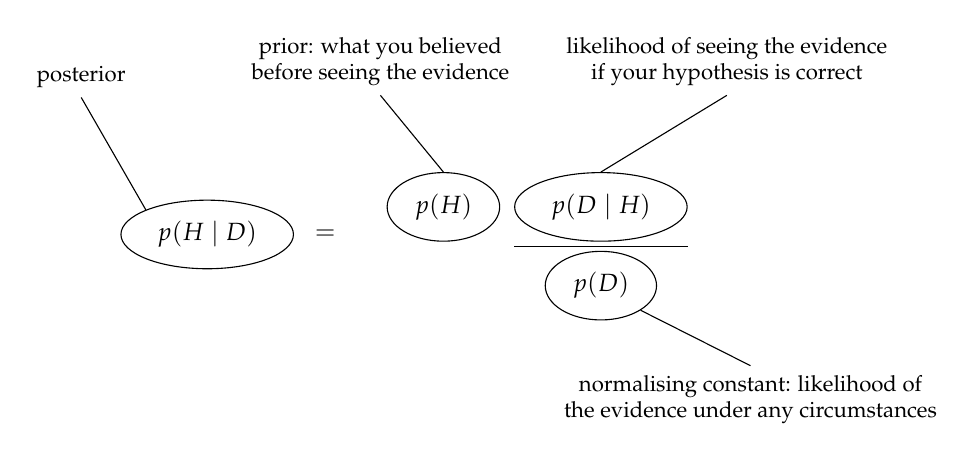
\begin{tikzpicture}[font=\small,>=Stealth]
  \node[draw,ellipse,inner sep=4pt] (post) at (0,0) {$p(H\mid D)$};
  \node at (1.5,0) {$=$};
  \node[draw,ellipse,inner sep=4pt] (prior) at (3.0,0.35) {$p(H)$};
  \node[draw,ellipse,inner sep=4pt] (lik) at (5.0,0.35) {$p(D\mid H)$};
  \draw (3.9,-0.15) -- (6.1,-0.15);
  \node[draw,ellipse,inner sep=4pt] (ev) at (5.0,-0.65) {$p(D)$};
  \node[align=center,font=\footnotesize] (t1) at (-1.6,2.0) {posterior};
  \node[align=center,font=\footnotesize] (t2) at (2.2,2.2) {prior: what you believed\\before seeing the evidence};
  \node[align=center,font=\footnotesize] (t3) at (6.6,2.2) {likelihood of seeing the evidence\\if your hypothesis is correct};
  \node[align=center,font=\footnotesize] (t4) at (6.9,-2.1) {normalising constant: likelihood of\\the evidence under any circumstances};
  \draw (t1.south) -- (post.north west);  \draw (t2.south) -- (prior.north);
  \draw (t3.south) -- (lik.north);        \draw (t4.north) -- (ev.south east);
\end{tikzpicture}
\caption{The annotated Bayes formula of slide 37.}
\end{figure}

\begin{intuition}
Posterior $\propto$ prior $\times$ likelihood; $p(D)$ only renormalises. Example: an ad is either \emph{good} (CTR $0.6$) or \emph{bad} (CTR $0.4$), prior $50/50$. After observing one click,
$p(\text{good}\mid\text{click})=\frac{0.5\cdot0.6}{0.5\cdot0.6+0.5\cdot0.4}=0.6$; after two clicks the odds multiply by $0.6/0.4$ again, giving odds $2.25$, i.e.\ $p\approx0.69$.
Each observation nudges belief towards the hypotheses that explain it best. This is the engine of Bayesian bandits.
\end{intuition}

% =====================================================================
\section{Bayesian Bandits \slides{38}}

So far we made \emph{no assumption} about the reward distributions $\nu_i$; we only derived bounds that hold for any bounded rewards. In \textbf{Bayesian bandits}:
\begin{itemize}
 \item we exploit \emph{prior} knowledge of the rewards;
 \item we update a \emph{posterior} distribution of rewards from the history;
 \item we use the posterior to guide exploration, via \textbf{upper confidence bounds} (Bayesian UCB) or \textbf{probability matching} (Thompson sampling).
\end{itemize}

\begin{intuition}
A frequentist guarantee protects you against \emph{any} reward distribution but is therefore conservative; a Bayesian method gets a head start when the prior is sensible (e.g.\ CTRs are mostly small) and the posterior directly
tells you ``how sure am I about each arm''. The price is that the guarantee is only as good as the modelling assumptions.
\end{intuition}

% =====================================================================
\section{Gaussian Bayesian Bandits Example \slides{39--40}}

\subsection{Setting \slides{39}}

Assume each reward distribution is Gaussian, $\nu_i=\Norm(\mu(i),\sigma^2(i))$. After some pulls the learner holds, for each arm, a belief (a Gaussian) about that arm's quality: the centre is the best guess
$\mu(i)$ and the width reflects remaining uncertainty.

\begin{figure}[ht]
\centering
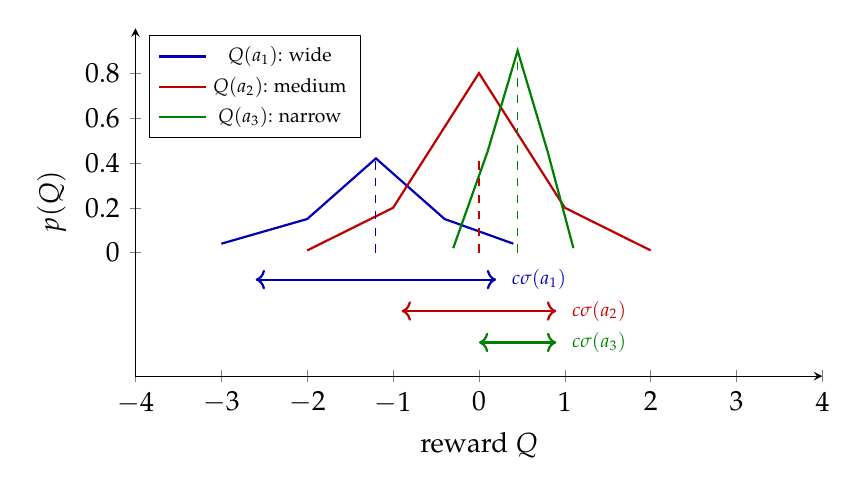
\begin{tikzpicture}
\begin{axis}[width=0.85\linewidth,height=6cm,xmin=-4,xmax=4,ymin=-0.55,ymax=1.0,xlabel={reward $Q$},ylabel={$p(Q)$},
  ytick={0,0.2,0.4,0.6,0.8},no markers,legend style={font=\scriptsize,at={(0.02,0.98)},anchor=north west},axis lines=left,clip=false]
 \addplot[blue!70!black,thick] coordinates {(-3,0.04) (-2,0.15) (-1.2,0.42) (-0.4,0.15) (0.4,0.04)};
 \addplot[red!75!black,thick] coordinates {(-2,0.01) (-1,0.20) (0,0.80) (1,0.20) (2,0.01)};
 \addplot[green!50!black,thick] coordinates {(-0.3,0.02) (0.1,0.45) (0.45,0.90) (0.8,0.45) (1.1,0.02)};
 \addlegendentry{$Q(a_1)$: wide}
 \addlegendentry{$Q(a_2)$: medium}
 \addlegendentry{$Q(a_3)$: narrow}
 \draw[dashed,blue!70!black] (axis cs:-1.2,0) -- (axis cs:-1.2,0.42);
 \draw[dashed,red!75!black] (axis cs:0,0) -- (axis cs:0,0.42);
 \draw[dashed,green!50!black] (axis cs:0.45,0) -- (axis cs:0.45,0.9);
 \draw[<->,blue!70!black,thick] (axis cs:-2.6,-0.12) -- (axis cs:0.2,-0.12) node[right,font=\scriptsize,xshift=2pt] {$c\sigma(a_1)$};
 \draw[<->,red!75!black,thick]  (axis cs:-0.9,-0.26) -- (axis cs:0.9,-0.26) node[right,font=\scriptsize,xshift=2pt] {$c\sigma(a_2)$};
 \draw[<->,green!50!black,thick](axis cs:0.0,-0.40) -- (axis cs:0.9,-0.40) node[right,font=\scriptsize,xshift=2pt] {$c\sigma(a_3)$};
\end{axis}
\end{tikzpicture}
\caption{Beliefs over the quality of three arms (slide 39 redrawn; dashed lines mark the means $\mu(a_i)$; the double arrows are confidence widths $\pm c\sigma$ around each mean). Arm~1 is very uncertain, arm~3 is well known.}
\end{figure}

\subsection{Posterior update \slides{40}}

The prior is often $\Norm(0,1)$. The posterior after history $h_t$ is proportional to the prior times the product of the likelihoods of all the rewards observed when this arm was selected (slide 40: ``product over all time-steps $t$ that select action $i$''). For a Gaussian prior and Gaussian noise this has a closed form.

\begin{proposition}[Gaussian conjugacy]\label{prop:gauss}
Let the unknown mean of an arm have prior $\mu\sim\Norm(m_0,s_0^2)$, and let $r_1,\dots,r_n$ be i.i.d.\ $\Norm(\mu,\sigma^2)$ with $\sigma^2$ known. Then the posterior is $\Norm(m_n,s_n^2)$ with
\[
 \frac1{s_n^2}=\frac1{s_0^2}+\frac n{\sigma^2},\qquad m_n=s_n^2\Bigl(\frac{m_0}{s_0^2}+\frac1{\sigma^2}\sum_{i=1}^nr_i\Bigr).
\]
\end{proposition}
\begin{proof}
By Bayes' rule (Theorem~\ref{thm:bayes}) the posterior density is proportional to prior times likelihood,
\[
 p(\mu\mid r_{1:n})\propto\exp\Bigl(-\frac{(\mu-m_0)^2}{2s_0^2}\Bigr)\prod_{i=1}^n\exp\Bigl(-\frac{(r_i-\mu)^2}{2\sigma^2}\Bigr).
\]
The exponent is a quadratic in $\mu$; collecting terms,
\[
 -\frac12\Bigl[\mu^2\Bigl(\frac1{s_0^2}+\frac n{\sigma^2}\Bigr)-2\mu\Bigl(\frac{m_0}{s_0^2}+\frac{\sum_ir_i}{\sigma^2}\Bigr)\Bigr]+\text{const},
\]
which is $-\frac1{2s_n^2}(\mu-m_n)^2+\text{const}$ for exactly the $s_n^2$ and $m_n$ of the statement. A density proportional to a Gaussian kernel is that Gaussian.
\end{proof}

\begin{corollary}[One-step update]\label{cor:gauss-step}
If arm $i$ has the posterior $\Norm(\mu_{t-1}(i),\sigma_{t-1}^2(i))$ and is pulled, yielding $r_t$, its new posterior is $\Norm(\mu_t(i),\sigma_t^2(i))$ with
\[
 \frac1{\sigma_t^2(i)}=\frac1{\sigma_{t-1}^2(i)}+\frac1{\sigma^2},\qquad
 \mu_t(i)=\sigma_t^2(i)\Bigl(\frac{\mu_{t-1}(i)}{\sigma_{t-1}^2(i)}+\frac{r_t}{\sigma^2}\Bigr);
\]
the posteriors of the other arms are unchanged.
\end{corollary}
\begin{proof}
Posterior updating can be done one observation at a time: the old posterior plays the role of the prior and Proposition~\ref{prop:gauss} is applied with $n=1$. Arms not pulled provide no data about their own mean, so their posteriors stay the same.
\end{proof}

This is the compact update shown on slide 40, $p(\mu_t(i),\sigma_t^2(i)\mid r_t)\propto p(\mu,\sigma^2)\,\Norm(r_t\mid\cdot)$: the slide writes the Gaussian likelihood of the new reward with the current posterior parameters as shorthand; the closed form above is what is actually computed.

\begin{figure}[ht]
\centering
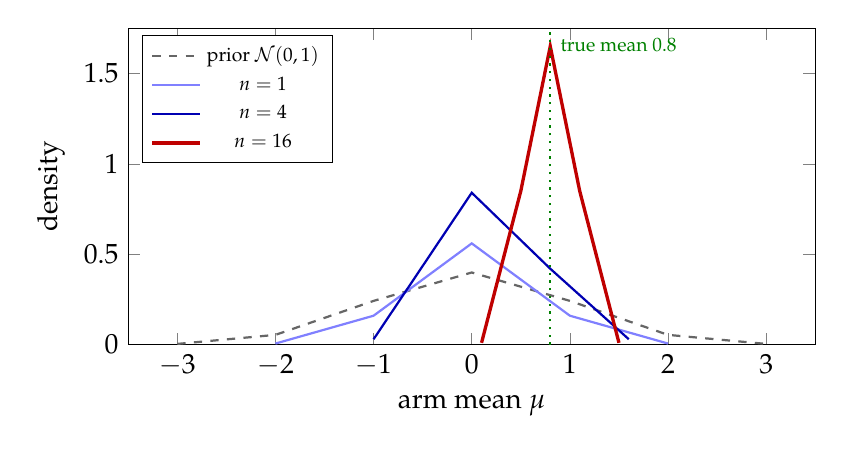
\begin{tikzpicture}
\begin{axis}[width=0.85\linewidth,height=5.6cm,xmin=-3.5,xmax=3.5,ymin=0,ymax=1.75,xlabel={arm mean $\mu$},ylabel={density},
 no markers,legend style={font=\scriptsize,at={(0.02,0.98)},anchor=north west}]
 \addplot[black!60,thick,dashed] coordinates {(-3,0.004) (-2,0.054) (-1,0.242) (0,0.399) (1,0.242) (2,0.054) (3,0.004)};
 \addplot[blue!50,thick] coordinates {(-2,0.006) (-1,0.16) (0,0.56) (1,0.16) (2,0.006)};
 \addplot[blue!70!black,thick] coordinates {(-1,0.03) (0,0.84) (0.8,0.42) (1.6,0.03)};
 \addplot[red!75!black,very thick] coordinates {(0.1,0.01) (0.5,0.85) (0.8,1.65) (1.1,0.85) (1.5,0.01)};
 \draw[dotted,thick,green!50!black] (axis cs:0.8,0) -- (axis cs:0.8,1.75) node[below right,font=\scriptsize] {true mean $0.8$};
 \addlegendentry{prior $\Norm(0,1)$}
 \addlegendentry{$n=1$}
 \addlegendentry{$n=4$}
 \addlegendentry{$n=16$}
\end{axis}
\end{tikzpicture}
\caption{Toy simulation of Proposition~\ref{prop:gauss} ($\sigma=1$, true mean $0.8$, seeded data): the posterior narrows like $1/\sqrt n$ (standard deviations $1,\ 0.71,\ 0.45,\ 0.24$ for $n=0,1,4,16$) and its centre drifts from the prior mean $0$ towards the truth
(posterior means $0.00$, $0.25$, $0.66$ for $n=1,4,16$ in this run).}
\end{figure}

\begin{intuition}
Precisions (inverse variances) \emph{add}: prior precision $1/s_0^2$ plus $1/\sigma^2$ per observation, and the posterior mean is a precision-weighted average of the prior mean and the data.
Worked example: prior $\Norm(0,1)$, $\sigma^2=1$, and $n=4$ observations summing to $3$. Then $s_4^2=1/(1+4)=0.2$ and $m_4=0.2\cdot(0+3)=0.6$: the sample mean $0.75$ is pulled slightly toward the prior mean~$0$ (like having one extra ``virtual'' observation equal to $0$).
The more data an arm has, the less the prior matters, and a rarely tried arm keeps a wide posterior, which is exactly what the exploration rules below exploit.
\end{intuition}

% =====================================================================
\section{Gaussian Bayesian Bandits: UCB \slides{41--43}}

Since we are modelling a distribution, we already have a measure of confidence. What is confidence for a Gaussian? Its \emph{standard deviation}. The slide proposes a UCB rule built from it:

\begin{algorithm}[Bayesian UCB (Gaussian)]\label{alg:bucb}
At round $t$ play
\[
 a_t=\argmax_{i\in[K]}\ \Bigl(\mu_t(i)+\frac{c\,\sigma_t(i)}{\sqrt{N_t(i)}}\Bigr),
\]
where $\mu_t(i)$ is the posterior mean, $N_t(i)$ the number of pulls of arm $i$, $\sigma_t(i)$ the Gaussian's standard deviation parameter and $c>0$ a constant that sets how optimistic we are.
\end{algorithm}

The slide's wording ``select the action with highest standard deviation'' is shorthand: the score is the mean plus $c$ times the uncertainty of the mean, $\sigma_t(i)/\sqrt{N_t(i)}$, which is the standard error of the arm's mean
(with a weak prior it coincides with the posterior standard deviation from Proposition~\ref{prop:gauss}).

\begin{figure}[ht]
\centering
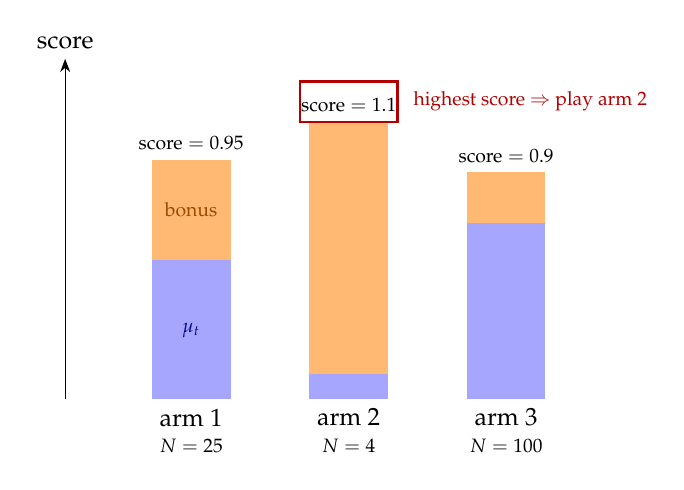
\begin{tikzpicture}[font=\small,>=Stealth,y=3.2cm]
  \draw[->] (-0.6,0) -- (-0.6,1.35) node[above] {score};
  \foreach \x/\mmu/\bon/\nn/\lab in {1/0.55/0.40/25/{$N=25$},3/0.10/1.00/4/{$N=4$},5/0.70/0.20/100/{$N=100$}}{
    \fill[blue!35] (\x-0.5,0) rectangle (\x+0.5,\mmu);
    \fill[orange!55] (\x-0.5,\mmu) rectangle (\x+0.5,\mmu+\bon);
    \node[below] at (\x,0) {arm \the\numexpr(\x+1)/2\relax};
    \node[below=11pt,font=\scriptsize] at (\x,0) {\lab};
    \pgfmathparse{\mmu+\bon}\let\score\pgfmathresult
    \node[above,font=\scriptsize] at (\x,\mmu+\bon) {$\mathrm{score}=\pgfmathprintnumber[fixed,precision=2]{\score}$};
  }
  \draw[red!70!black,thick] (3-0.62,1.10) rectangle (3+0.62,1.26);
  \node[blue!50!black,font=\scriptsize] at (1,0.27) {$\mu_t$};  \node[orange!60!black,font=\scriptsize] at (1,0.75) {bonus};
  \node[red!70!black,font=\scriptsize,right] at (3.7,1.18) {highest score $\Rightarrow$ play arm 2};
\end{tikzpicture}
\caption{Snapshot of Algorithm~\ref{alg:bucb} with $c=2$, $\sigma=1$ (illustrative numbers). Blue: posterior mean; orange: bonus $c\sigma/\sqrt{N}$. Arm~2 has the \emph{lowest} mean but is almost unexplored, so its bonus ($1.0$) lifts it to the top.}
\end{figure}

\begin{intuition}
Compare with Algorithm~\ref{alg:ucb}: the distribution-free width $\sqrt{\ln(KT/\delta)/N}$ is replaced by $c\sigma/\sqrt N$, with $c$ playing the role of $\sqrt{\ln(KT/\delta)}$. Under a Gaussian belief, $c=2$ means that the true mean lies below the score with probability
$\Phi(2)\approx97.7\%$. In the snapshot (means $0.55,0.10,0.70$; counts $25,4,100$; $c=2$) the scores are $0.95,\ 1.10,\ 0.90$: the well-explored best-looking arm is passed over in favour of the least-explored one, as optimism demands.
Slide 43 shows an animation of the rule: as an arm is pulled its bonus shrinks, so the scores converge towards the true means and the choice settles on the best arm.
\end{intuition}
% =====================================================================
\section{Gaussian Bayesian Bandits: Thompson Sampling \slides{44--48}}

\subsection{Probability matching \slides{44--45}}

Thompson sampling (TS) is a way to do \emph{probability matching}: it selects an action with probability equal (or proportional) to the probability that the action is optimal given what we know, i.e.\ its \emph{posterior probability of being optimal}.
It is optimistic in the face of uncertainty, because uncertain actions have a higher probability of attaining the maximum, and it \emph{uses sampling to avoid the complications of actual probability matching}.

\emph{Slide example.} You are choosing between two ads. Each step you draw a plausible click-through rate for A and for B from your current beliefs, show the ad with the higher draw, observe the result and update your beliefs; the truly better ad is picked more and more over time.

\begin{algorithm}[Thompson sampling (posterior sampling)]\label{alg:ts}
For $t=0,1,\dots,T-1$:
\begin{enumerate}
 \item for each arm $a$, draw $\tilde\mu_t(a)$ \emph{independently} from the current posterior of $\mu(a)$;
 \item play $A_t\in\argmax_a\tilde\mu_t(a)$;
 \item observe $r_t$ and update the posterior of arm $A_t$ only.
\end{enumerate}
In the contextual case the posterior is over the parameters of the \emph{reward model}: step~1 draws one model, and step~2 acts greedily with respect to that draw.
\end{algorithm}

\begin{proposition}[Thompson sampling is probability matching]\label{prop:pm}
Assume the arms' means are independent under the posterior given the history $h_t$. Then for every arm $a$ (ties broken by the same rule on both sides)
\[
 \Prob(A_t=a\mid h_t)=\Prob\bigl(a\in\argmax_{a'}\mu(a')\bigm|h_t\bigr),
\]
i.e.\ the algorithm plays each arm exactly as often as it believes that arm is optimal.
\end{proposition}
\begin{proof}
By independence, drawing $\tilde\mu_t(a)$ from each arm's marginal posterior independently is a draw of the whole vector $\tilde\mu_t$ from the joint posterior of $(\mu(1),\dots,\mu(K))$ given $h_t$.
The event $\{A_t=a\}$ is the event $\{a\in\argmax_{a'}\tilde\mu_t(a')\}$, whose probability under the joint posterior is by definition the posterior probability that $a$ is an optimal arm.
\end{proof}

\begin{figure}[ht]
\centering
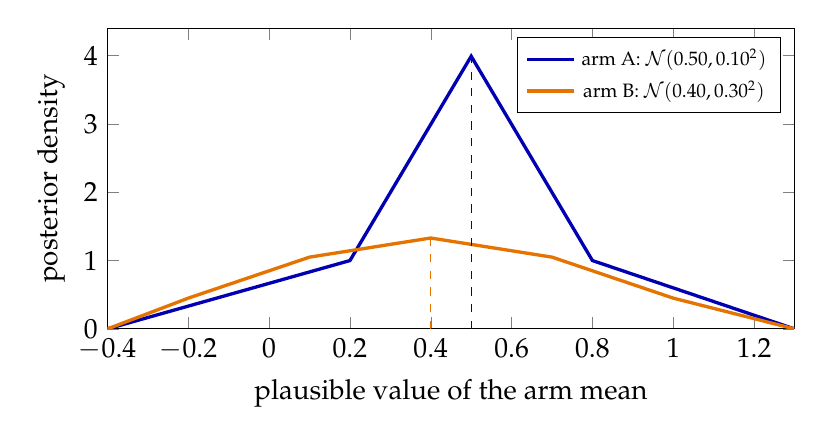
\begin{tikzpicture}
\begin{axis}[width=0.85\linewidth,height=5.4cm,xmin=-0.4,xmax=1.3,ymin=0,ymax=4.4,xlabel={plausible value of the arm mean},ylabel={posterior density},
  no markers,legend style={font=\scriptsize,at={(0.98,0.97)},anchor=north east}]
 \addplot[blue!70!black,very thick] coordinates {(-0.4,0.00) (0.2,1.0) (0.5,3.99) (0.8,1.0) (1.3,0.00)};
 \addplot[orange!90!black,very thick] coordinates {(-0.4,0.00) (-0.2,0.45) (0.1,1.05) (0.4,1.33) (0.7,1.05) (1.0,0.45) (1.3,0.00)};
 \addlegendentry{arm A: $\Norm(0.50,0.10^2)$}
 \addlegendentry{arm B: $\Norm(0.40,0.30^2)$}
 \draw[dashed,blue!70!black] (axis cs:0.5,0) -- (axis cs:0.5,3.99);
 \draw[dashed,orange!90!black] (axis cs:0.4,0) -- (axis cs:0.4,1.33);
\end{axis}
\end{tikzpicture}
\caption{Two posteriors with independent arms. A has the higher mean but B is much more uncertain; B's posterior probability of being the better arm is $\Phi\bigl(-0.1/\sqrt{0.1^2+0.3^2}\bigr)\approx0.376$, so TS plays B about 37.6\% of the time.}
\end{figure}

\begin{intuition}
Why ``sample, then argmax'' (slide 45) is enough: you never compute $\Prob(\text{arm }a\text{ is best})$ explicitly; you just \emph{simulate one possible world} consistent with your beliefs and act optimally in it. Over many rounds the frequency with which each arm wins its
simulated world is precisely its probability of being optimal. In the figure, for independent Gaussians $\Prob(\mu_B>\mu_A)=\Phi\bigl((m_B-m_A)/\sqrt{s_A^2+s_B^2}\bigr)=\Phi(-0.316)\approx0.376$ (a Monte Carlo check with $10^6$ pairs of draws gives $0.375$). The less-known arm keeps getting tried
\emph{in proportion to how plausibly it might be best}; once its posterior narrows below the other arm's, that probability collapses to zero and exploration stops by itself.
\end{intuition}

\subsection{The Gaussian algorithm \slides{46--47}}

\begin{algorithm}[Thompson sampling, Gaussian arms]\label{alg:tsg}
For $t=0,\dots,T$:
\begin{enumerate}
 \item for each arm $i=1,\dots,K$ sample a value $\tilde\mu_t(i)$ \emph{independently} from $\Norm\bigl(\mu_{t-1}(i),\sigma^2_{t-1}(i)\bigr)$ (the slides denote this sampled value by $\hat{\mathbf r}_i$; it is \emph{not} the IPS vector of Section~5);
 \item pull the arm $I_t=\argmax_{i\in[K]}\tilde\mu_t(i)$;
 \item observe the reward $r_t$;
 \item update the posterior of the pulled arm via Corollary~\ref{cor:gauss-step}.
\end{enumerate}
\end{algorithm}

Slide 47 adds two remarks. First, the sampled value is an estimate of the \emph{reward}; in a general MDP it can be replaced by the $Q$-function, i.e.\ we estimate a \emph{distribution over $Q$} and sample from it.
Second, ``this can be done with different distributions as well'' (see Section~\ref{sec:beta}).

\begin{intuition}
Compared with Bayesian UCB, nothing is added to the mean: uncertainty enters \emph{through the randomness of the sample}. A wide posterior occasionally produces a very high draw and so gets tried; a narrow posterior almost always draws close to its mean. This ``randomised optimism''
needs no tuning constant $c$, only a sensible prior.
\end{intuition}

\subsection{Simulation \slides{48}}

\begin{figure}[ht]
\centering
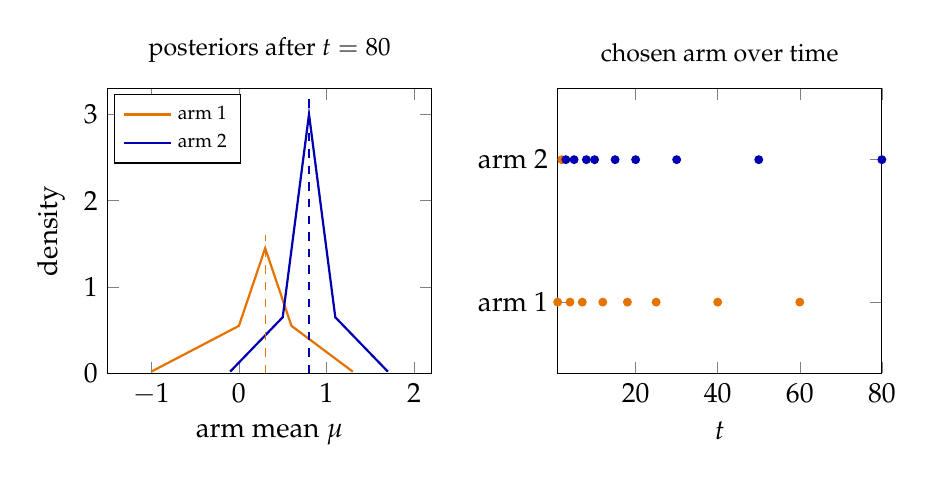
\begin{tikzpicture}
\begin{groupplot}[group style={group size=2 by 1,horizontal sep=1.6cm},width=0.47\linewidth,height=5.2cm,no markers,title style={font=\small}]
 \nextgroupplot[title={posteriors after $t=80$},xlabel={arm mean $\mu$},ylabel={density},xmin=-1.5,xmax=2.2,ymin=0,
   legend style={font=\scriptsize,at={(0.02,0.98)},anchor=north west}]
  \addplot[orange!90!black,thick] coordinates {(-1.0,0.02) (0.0,0.55) (0.3,1.45) (0.6,0.55) (1.3,0.02)};
  \addplot[blue!70!black,thick] coordinates {(-0.1,0.02) (0.5,0.65) (0.8,3.0) (1.1,0.65) (1.7,0.02)};
  \draw[dashed,orange!90!black] (axis cs:0.3,0) -- (axis cs:0.3,1.6);
  \draw[dashed,blue!70!black] (axis cs:0.8,0) -- (axis cs:0.8,3.2);
  \addlegendentry{arm 1}
 \addlegendentry{arm 2}
 \nextgroupplot[title={chosen arm over time},xlabel={$t$},xmin=1,xmax=80,ymin=0.5,ymax=2.5,ytick={1,2},yticklabels={arm 1,arm 2}]
  \addplot[only marks,mark=*,mark size=1.4pt,orange!90!black] coordinates {(1,1) (2,2) (4,1) (7,1) (12,1) (18,1) (25,1) (40,1) (60,1)};
  \addplot[only marks,mark=*,mark size=1.4pt,blue!70!black] coordinates {(3,2) (5,2) (8,2) (10,2) (15,2) (20,2) (30,2) (50,2) (80,2)};
\end{groupplot}
\end{tikzpicture}
\caption{Toy simulation of Algorithm~\ref{alg:tsg} (seeded): two Gaussian arms with true means $0.3$ and $0.8$ (dashed), noise $\sigma=1$, prior $\Norm(0,1)$, $T=80$. Arm~1 is tried 13 times and then largely abandoned; arm~2 is played in 67 rounds.
Final posteriors: arm~1 $\Norm(0.22,0.27^2)$ (still wide, as it was rarely sampled), arm~2 $\Norm(0.69,0.12^2)$ (narrow).}
\end{figure}

% =====================================================================
\section{Bayesian Bandits: Thompson Sampling \slides{49}}\label{sec:beta}

Slide 49 repeats the algorithm with \emph{Beta posteriors} for an A/B ad test (click-through rates in $[0,1]$). Each step: sample $\tilde\theta_A,\tilde\theta_B$ from the Beta posteriors, pick the argmax, observe a click, and update that arm only.

\begin{proposition}[Beta--Bernoulli conjugacy]\label{prop:beta}
If $\mu\sim\mathrm{Beta}(\alpha,\beta)$ and $r\sim\mathrm{Bernoulli}(\mu)$, then $\mu\mid r\sim\mathrm{Beta}(\alpha+r,\ \beta+1-r)$. After $k$ successes in $n$ trials from the uniform prior $\mathrm{Beta}(1,1)$, the posterior is $\mathrm{Beta}(1+k,\,1+n-k)$, with mean $\frac{k+1}{n+2}$ and variance $\frac{\alpha\beta}{(\alpha+\beta)^2(\alpha+\beta+1)}$ (with $\alpha=1+k$, $\beta=1+n-k$).
\end{proposition}
\begin{proof}
The Beta density is proportional to $\mu^{\alpha-1}(1-\mu)^{\beta-1}$ and the Bernoulli likelihood is $\mu^r(1-\mu)^{1-r}$. Their product is proportional to $\mu^{\alpha+r-1}(1-\mu)^{\beta+(1-r)-1}$, the kernel of $\mathrm{Beta}(\alpha+r,\beta+1-r)$.
Iterating $n$ times adds the successes to $\alpha$ and the failures to $\beta$; the moments are those of the Beta distribution.
\end{proof}

\begin{algorithm}[Thompson sampling, Bernoulli rewards]
Keep $(\alpha_i,\beta_i)=(1,1)$ for each arm $i$. At each round: draw $\tilde\theta_i\sim\mathrm{Beta}(\alpha_i,\beta_i)$ for all $i$, play $I_t=\argmax_i\tilde\theta_i$, observe the click $c_t\in\{0,1\}$, and set $\alpha_{I_t}\leftarrow\alpha_{I_t}+c_t$, $\beta_{I_t}\leftarrow\beta_{I_t}+1-c_t$.
\end{algorithm}

\begin{figure}[ht]
\centering
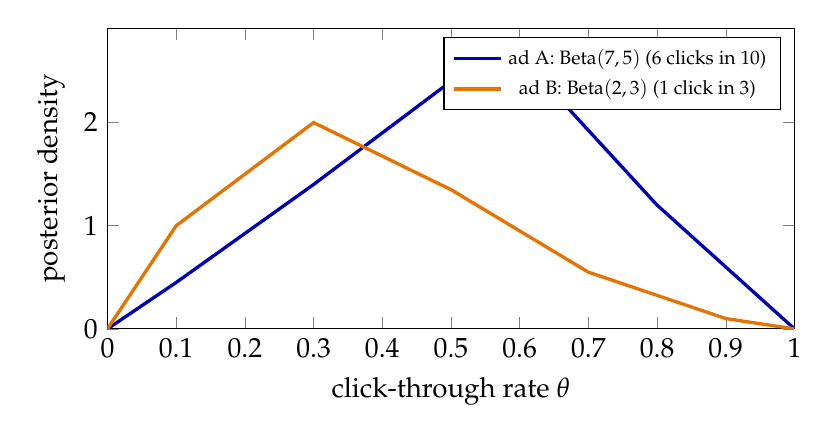
\begin{tikzpicture}
\begin{axis}[width=0.85\linewidth,height=5.4cm,xmin=0,xmax=1,ymin=0,xlabel={click-through rate $\theta$},ylabel={posterior density},no markers,
  legend style={font=\scriptsize,at={(0.98,0.97)},anchor=north east}]
 \addplot[blue!70!black,very thick] coordinates {(0,0) (0.1,0.45) (0.3,1.4) (0.5,2.4) (0.6,2.65) (0.8,1.2) (1,0)};
 \addplot[orange!90!black,very thick] coordinates {(0,0) (0.1,1.0) (0.3,2.0) (0.5,1.35) (0.7,0.55) (0.9,0.1) (1,0)};
 \addlegendentry{ad A: $\mathrm{Beta}(7,5)$ (6 clicks in 10)}
 \addlegendentry{ad B: $\mathrm{Beta}(2,3)$ (1 click in 3)}
\end{axis}
\end{tikzpicture}
\caption{Beta posteriors for an A/B test from the uniform prior (illustrative counts). Ad B has little data, so its posterior is broad.}
\end{figure}

\begin{intuition}
Beta--Bernoulli is the Bernoulli analogue of Proposition~\ref{prop:gauss}: ``pseudo-counts'' of successes and failures. For ad A ($k=6$, $n=10$): mean $7/12\approx0.583$, variance $\approx0.0187$. For ad B ($k=1$, $n=3$): mean $2/5=0.4$, variance $0.04$.
The probability that a draw for A beats a draw for B is $\approx0.77$ (Monte Carlo, $10^6$ draws), so Thompson sampling would show A about 77\% of the time and still B about 23\% of the time, because B's few observations leave
real doubt. Each click or non-click then moves the corresponding posterior and the shares drift towards the truly better ad. This is the ``different distributions'' remark of slides 47 and 49: the algorithm only needs a posterior one can \emph{sample} from.
\end{intuition}

% =====================================================================
\section{Summary}

\begin{table}[ht]
\centering\small
\renewcommand{\arraystretch}{1.25}
\begin{tabular}{>{\raggedright\arraybackslash}p{2.2cm}>{\raggedright\arraybackslash}p{1.35cm}>{\raggedright\arraybackslash}p{3.9cm}>{\raggedright\arraybackslash}p{2.4cm}>{\raggedright\arraybackslash}p{4.05cm}}
\toprule
\textbf{Method} & \textbf{Setting} & \textbf{How it explores} & \textbf{Assumes} & \textbf{Result in this lecture}\\\midrule
Greedy & MAB & try each arm once, commit to the best sample & nothing & linear regret (about $0.08T$ in the Bernoulli example)\\
Explore-then-commit & MAB & $N$ pulls per arm, then commit & rewards in $[0,1]$; needs $T,K,\delta$ to set $N$ & $O(T^{2/3}K^{1/3}\ln^{1/3}(K/\delta))$ (Thm.~\ref{thm:ec-mab})\\
UCB & MAB & optimism: mean $+\sqrt{\ln(KT/\delta)/N_t}$ & rewards in $[0,1]$ & $\widetilde O(\sqrt{KT})$, optimal up to logs (Thm.~\ref{thm:ucb})\\
Explore-then-commit & CB & uniform actions $+$ IPS for $N$ rounds, then $\hat\pi$ & finite $\Pi$ & $O\bigl(T^{2/3}K^{2/3}\ln^{1/3}(|\Pi|/\delta)\bigr)$ as proved (Thm.~\ref{thm:cec}); slide: $K^{1/3}$\\
$\epsilon$-greedy & CB & mixture $(1-\epsilon_t)\delta_{\pi^t}+\epsilon_t\Unif$ $+$ IPS, $\epsilon_t\downarrow0$ & finite/given $\Pi$ & no bound stated (simulation only)\\
Bayesian UCB & MAB (Gaussian) & posterior mean $+\,c\,\sigma_t/\sqrt{N_t}$ & Gaussian prior and noise & none stated (rule and snapshot)\\
Thompson sampling & MAB / CB & sample from posterior, act greedily on the sample & sampleable posterior (Gaussian, Beta, \dots) & plays arm $a$ with prob.\ $\Prob(a\text{ optimal})$ (Prop.~\ref{prop:pm}); no regret bound stated\\\bottomrule
\end{tabular}
\caption{Comparison of the methods covered. ``CB'' = contextual bandit, ``MAB'' = multi-armed bandit. ``None stated'' means neither the slides nor the companion note give a bound.}
\end{table}

\begin{figure}[ht]
\centering
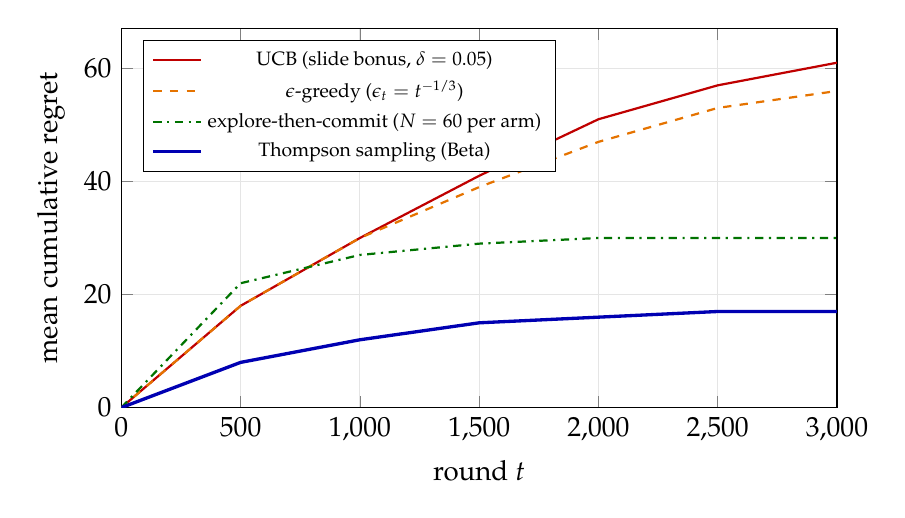
\begin{tikzpicture}
\begin{axis}[width=0.88\linewidth,height=6.4cm,xlabel={round $t$},ylabel={mean cumulative regret},xmin=0,xmax=3000,ymin=0,no markers,
  legend style={font=\scriptsize,at={(0.03,0.97)},anchor=north west},grid=both,grid style={black!10}]
 \addplot[red!75!black,thick] coordinates {(0,0) (500,18) (1000,30) (1500,41) (2000,51) (2500,57) (3000,61)};
 \addplot[orange!90!black,thick,dashed] coordinates {(0,0) (500,18) (1000,30) (1500,39) (2000,47) (2500,53) (3000,56)};
 \addplot[green!45!black,thick,dash dot] coordinates {(0,0) (500,22) (1000,27) (1500,29) (2000,30) (2500,30) (3000,30)};
 \addplot[blue!70!black,very thick] coordinates {(0,0) (500,8) (1000,12) (1500,15) (2000,16) (2500,17) (3000,17)};
 \addlegendentry{UCB (slide bonus, $\delta=0.05$)}
 \addlegendentry{$\epsilon$-greedy ($\epsilon_t=t^{-1/3}$)}
 \addlegendentry{explore-then-commit ($N=60$ per arm)}
 \addlegendentry{Thompson sampling (Beta)}
\end{axis}
\end{tikzpicture}
\caption{Toy simulation (qualitative): Bernoulli bandit with $K=3$ arms of means $0.7,0.5,0.4$, $T=3000$, regret averaged over 300 seeded runs. At $T=3000$ the average regrets are about $17$ (Thompson), $30$ (explore-then-commit), $56$ ($\epsilon$-greedy) and $61$ (UCB).
Constants matter in a short horizon: UCB with the conservative slide bonus $\sqrt{\ln(KT/\delta)/N}$ explores a lot, and explore-then-commit works well here only because $N=60$ was hand-picked (the theory needs the gaps, or $T,K,\delta$ and a bound, to choose it).
Asymptotically the ordering of \emph{rates} (linear $\gg T^{2/3}\gg\sqrt T$) is what the theorems describe.}
\end{figure}

\subsection*{Key take-aways}
\begin{itemize}
 \item \textbf{Exploration is unavoidable, and regret measures its price.} Greedy suffers linear regret; explore-then-commit balances exploration against commitment to get $T^{2/3}$; optimism (UCB) gets the optimal $\sqrt T$ rate up to logs, with no schedule to tune.
 \item \textbf{Context changes the object being learned, not the logic.} A contextual bandit asks for a \emph{policy}, with i.i.d.\ contexts and bandit feedback; regret is measured against the best policy in $\Pi$, and the cost of a rich class is only $\ln|\Pi|$ (inside a cube root).
 \item \textbf{IPS makes learning from partial feedback possible.} Dividing by the known propensity gives an unbiased estimate of every action's reward (Lemma~\ref{lem:ips}), at the price of variance up to $K$ (uniform exploration) or $K/\epsilon_t$ ($\epsilon$-greedy), which is why exploration probabilities must stay positive.
 \item \textbf{Explore-then-commit separates the phases, $\epsilon$-greedy interleaves them.} The first is easy to analyse (Theorem~\ref{thm:cec}); the second keeps learning and adapting but needs a decay schedule for $\epsilon_t$.
 \item \textbf{Bayesian bandits turn uncertainty into a distribution you can use.} Conjugate updates (Gaussian, Beta--Bernoulli) are one-line formulas; Bayesian UCB adds a multiple of the posterior width, while Thompson sampling samples from the posterior and thereby plays each arm with its probability of being optimal (Proposition~\ref{prop:pm}).
\end{itemize}

% =====================================================================
\appendix
\section{Supplementary material (in the companion note, not on the slides)}\label{app:supp}

The following result is in the companion note but has no corresponding slide; it supplies the technical ingredient (range of the IPS terms) used in the proof of Theorem~\ref{thm:cec}.

\begin{lemma}[What unbiasedness costs]\label{lem:range}
Under uniform exploration, $0\le\rh_t[a]\le K$ and $\Var\bigl(\rh_t[a]\mid x_t\bigr)\le K$.
\end{lemma}
\begin{proof}
The estimator is $Kr_t\le K$ on one action and $0$ elsewhere, which gives the range. For the variance,
$\E[\rh_t[a]^2\mid x_t]=\frac1K\,K^2\,\E[r_t^2\mid x_t,a]\le K$, since rewards lie in $[0,1]$, and the variance is at most the second moment.
\end{proof}

\begin{intuition}
Unbiasedness is bought with noise: each observation is $0$ with probability $1-1/K$ and $Kr_t$ with probability $1/K$. With $K=10$ actions and reward $0.5$, a single IPS observation is either $0$ or $5$ although the target is $0.5$; its variance is $10\cdot0.25-0.25=2.25$, versus at most $0.25$ for a $[0,1]$-valued observation.
The \emph{range} bound $K$ is what Hoeffding's inequality uses in Theorem~\ref{thm:cec}; the \emph{variance} bound $K$ is what Bernstein's inequality would use to sharpen the dependence on $K$ (see the remark after that theorem).
\end{intuition}

\section{Notation map and slide/note discrepancies}\label{app:notes}

\begin{table}[ht]
\centering\small
\renewcommand{\arraystretch}{1.2}
\begin{tabular}{lll}\toprule
\textbf{Concept} & \textbf{Slides} & \textbf{Companion note / these notes}\\\midrule
context, context set & $x_t$, $\mathcal X$ & $z_t$, $\mathcal Z$ $\;/\;$ $x_t$, $\calX$\\
context distribution & $\mu$ & $\rho$\\
action at round $t$ & $a_t$ (CB), $I_t$ (MAB) & $A_t$ $\;/\;$ $a_t$, $I_t$\\
policy at round $t$ & $\pi^t$ & $\pi_t$\\
regret & $\mathrm{Regret}_T$ & $\mathrm{Reg}(T)$\\
IPS vector & $\hat{\mathbf r}_t[a]$ & $\hat r_t[a]$ $\;/\;$ $\rh_t[a]$\\\bottomrule
\end{tabular}
\end{table}

Small inconsistencies noticed while merging the two sources, and how these notes treat them:
\begin{itemize}
 \item \textbf{Slide 8:} ``Set $N=T/K$'' would use all $T$ rounds for exploration; read it as a placeholder with $NK\ll T$. The optimised $N^\star$ is on slide 12 and in Theorem~\ref{thm:ec-mab}.
 \item \textbf{Slide 12:} ``approaches 0 as $T$ goes to infinity'' refers to the \emph{average} regret $\Reg_T/T\sim T^{-1/3}$; the regret itself grows (sub-linearly).
 \item \textbf{Slides 11--12 and 14:} confidence widths are written with $\ln(K/\delta)$ or $\ln(KT/\delta)$, hiding the constant $2$ and Hoeffding's factor $\tfrac12$ inside $O(\cdot)$; the proofs here keep $\ln(2K/\delta)$ and $\ln(2KT/\delta)$.
 \item \textbf{Slide 31 vs.\ Theorem~\ref{thm:cec}:} slide $K^{1/3}$, proved bound $K^{2/3}$; see the remark after the theorem.
 \item \textbf{Slide 42:} ``highest standard deviation'' should read ``highest mean plus $c$ standard errors'', as the displayed formula says.
 \item \textbf{Slides 46--47:} the hat-bold-$r$ symbol there denotes a \emph{sample from the posterior}, unrelated to the IPS vector of slides 27--35.
 \item \textbf{Slide 40:} the recursive update is written with the likelihood evaluated at the current posterior parameters; the closed form is Corollary~\ref{cor:gauss-step}.
\end{itemize}

\end{document}